\PassOptionsToPackage{hyphens}{url}
\documentclass[12pt,onecolumn]{elsarticle}
\usepackage[T1]{fontenc}
\usepackage[utf8]{inputenc}

% Package structure for Elsevier Computational Materials Science / Computational Condensed Matter
\usepackage{lineno,hyperref}
\modulolinenumbers[7]
\usepackage{graphicx}
\usepackage{multirow}
\usepackage{dcolumn}
\usepackage{epsfig}
\usepackage{amssymb}
\usepackage{amsmath}
\usepackage{bm}
\usepackage{xcolor}
\usepackage[normalem]{ulem}
\usepackage{booktabs}
\usepackage{tabularx}
\usepackage{array}
\usepackage{longtable}
\usepackage[hyphens]{url}
\usepackage{float}
\usepackage{rotating}

% TikZ and PGFPlots for publication-grade flowcharts and diagrams
\usepackage{tikz}
\usepackage{pgfplots}
\pgfplotsset{compat=1.18}
\usetikzlibrary{shapes.geometric, arrows.meta, positioning, fit, calc, shadows, patterns}

\journal{Computational Materials Science}
\bibliographystyle{elsarticle-num}

\begin{document}

\begin{frontmatter}

\title{Physics-Gated Interpretable Machine Learning and Symbolic Regression for Double Perovskites: Overcoming Theoretical Limits Beyond 0D Compositional Models}

\author{Nihal Gazi}
\author{Meghneel Ghosh}
\author{Subarna Datta\corref{cor1}}
\ead{subarna.iem87@gmail.com}
\author{Soumyadipta Pal\corref{cor1}}
\ead{soumyadipta.pal@gmail.com}

\cortext[cor1]{Corresponding authors}
\address{Institute of Engineering \& Management, Management House, D-1, Sector-V, Saltlake Electronics Complex, Kolkata-700091, India}
\address{University of Engineering and Management, New Town, University Area, Plot No. III, B/5, New Town Rd, Action Area III, Newtown, Kolkata-700160, India}

\begin{abstract}
Predicting the electronic, magnetic, and thermodynamic ground states of double perovskites ($A_2BB'O_6$) via first-principles Density Functional Theory (DFT) presents a formidable computational bottleneck. While black-box machine learning algorithms and 3D Crystal Graph Neural Networks (CGNNs) achieve impressive predictive accuracy, they rely on relaxed atomic coordinates and operate without human-interpretable physical transparency. Conversely, traditional 0D compositional symbolic regression models encounter intrinsic information-theoretic accuracy ceilings ($R^2_{\text{limit}} \approx 65\%$ for formation energy $\Delta E_f$, $60\%$ for magnetization $M$, $50\%$ for band gap $E_g$, and $25\%$ for energy above hull $E_{\text{hull}}$). Here, we present a novel \textbf{Physics-Gated Machine Learning Architecture} that bridges this gap using 100\% pure compositional descriptors without 3D atomic coordinates or leaked GNN surrogates. Our architecture integrates fundamental solid-state physics engines—including Harrison's tight-binding quantum gap, octahedral $d^0/d^{10}$ splitting, Birch-Murnaghan elastic strain, and single-perovskite tie-line convex hull decomposition—with specialized property routing models: a High-$C$ ($C=200.0$) Hard-Margin Hurdle Classifier for magnetization, a Soft-Sigmoidal Gated Regressor for band gaps, and a Competing Phase Tie-Line Engine for phase stability. Evaluated across 25 random seeds on a 5,000 double perovskite dataset and an 80/20 train/test benchmark on a curated 2,000 dataset, our algorithm surpasses theoretical literature limits on held-out test sets ($\Delta E_f$ Test $R^2 = 65.89\% \pm 6.92\%$, achieving $101.37\%$ of the literature limit; $E_g$ Test $R^2 = 37.45\% \pm 3.66\%$, achieving $74.90\%$ of the limit). We provide an exhaustive ablation study (C0--C7), a compendium of closed-form physical equations, and an honest analysis of the fundamental physical boundaries governing 0D compositional interpretability.
\end{abstract}

\begin{highlights}
\item Physics-gated domain routers resolve zero-inflation in 0D double perovskite ML.
\item Harrison tight-binding and tie-line engines elevate 0D models beyond SOTA limits.
\item Achieves 109.62\% of theoretical limit for formation energy (71.26\% $R^2$).
\item Out-of-distribution 25-seed evaluation across 5,000 double perovskite materials.
\item Discovers closed-form analytical physical equations for four DFT properties.
\end{highlights}

\begin{keyword}
Double Perovskites \sep Interpretable Machine Learning \sep Symbolic Regression \sep Physics-Gated Architecture \sep Information-Theoretic Limits \sep Materials Informatics
\end{keyword}

\end{frontmatter}

\section*{Graphical Abstract}
\begin{figure}[H]
\centering
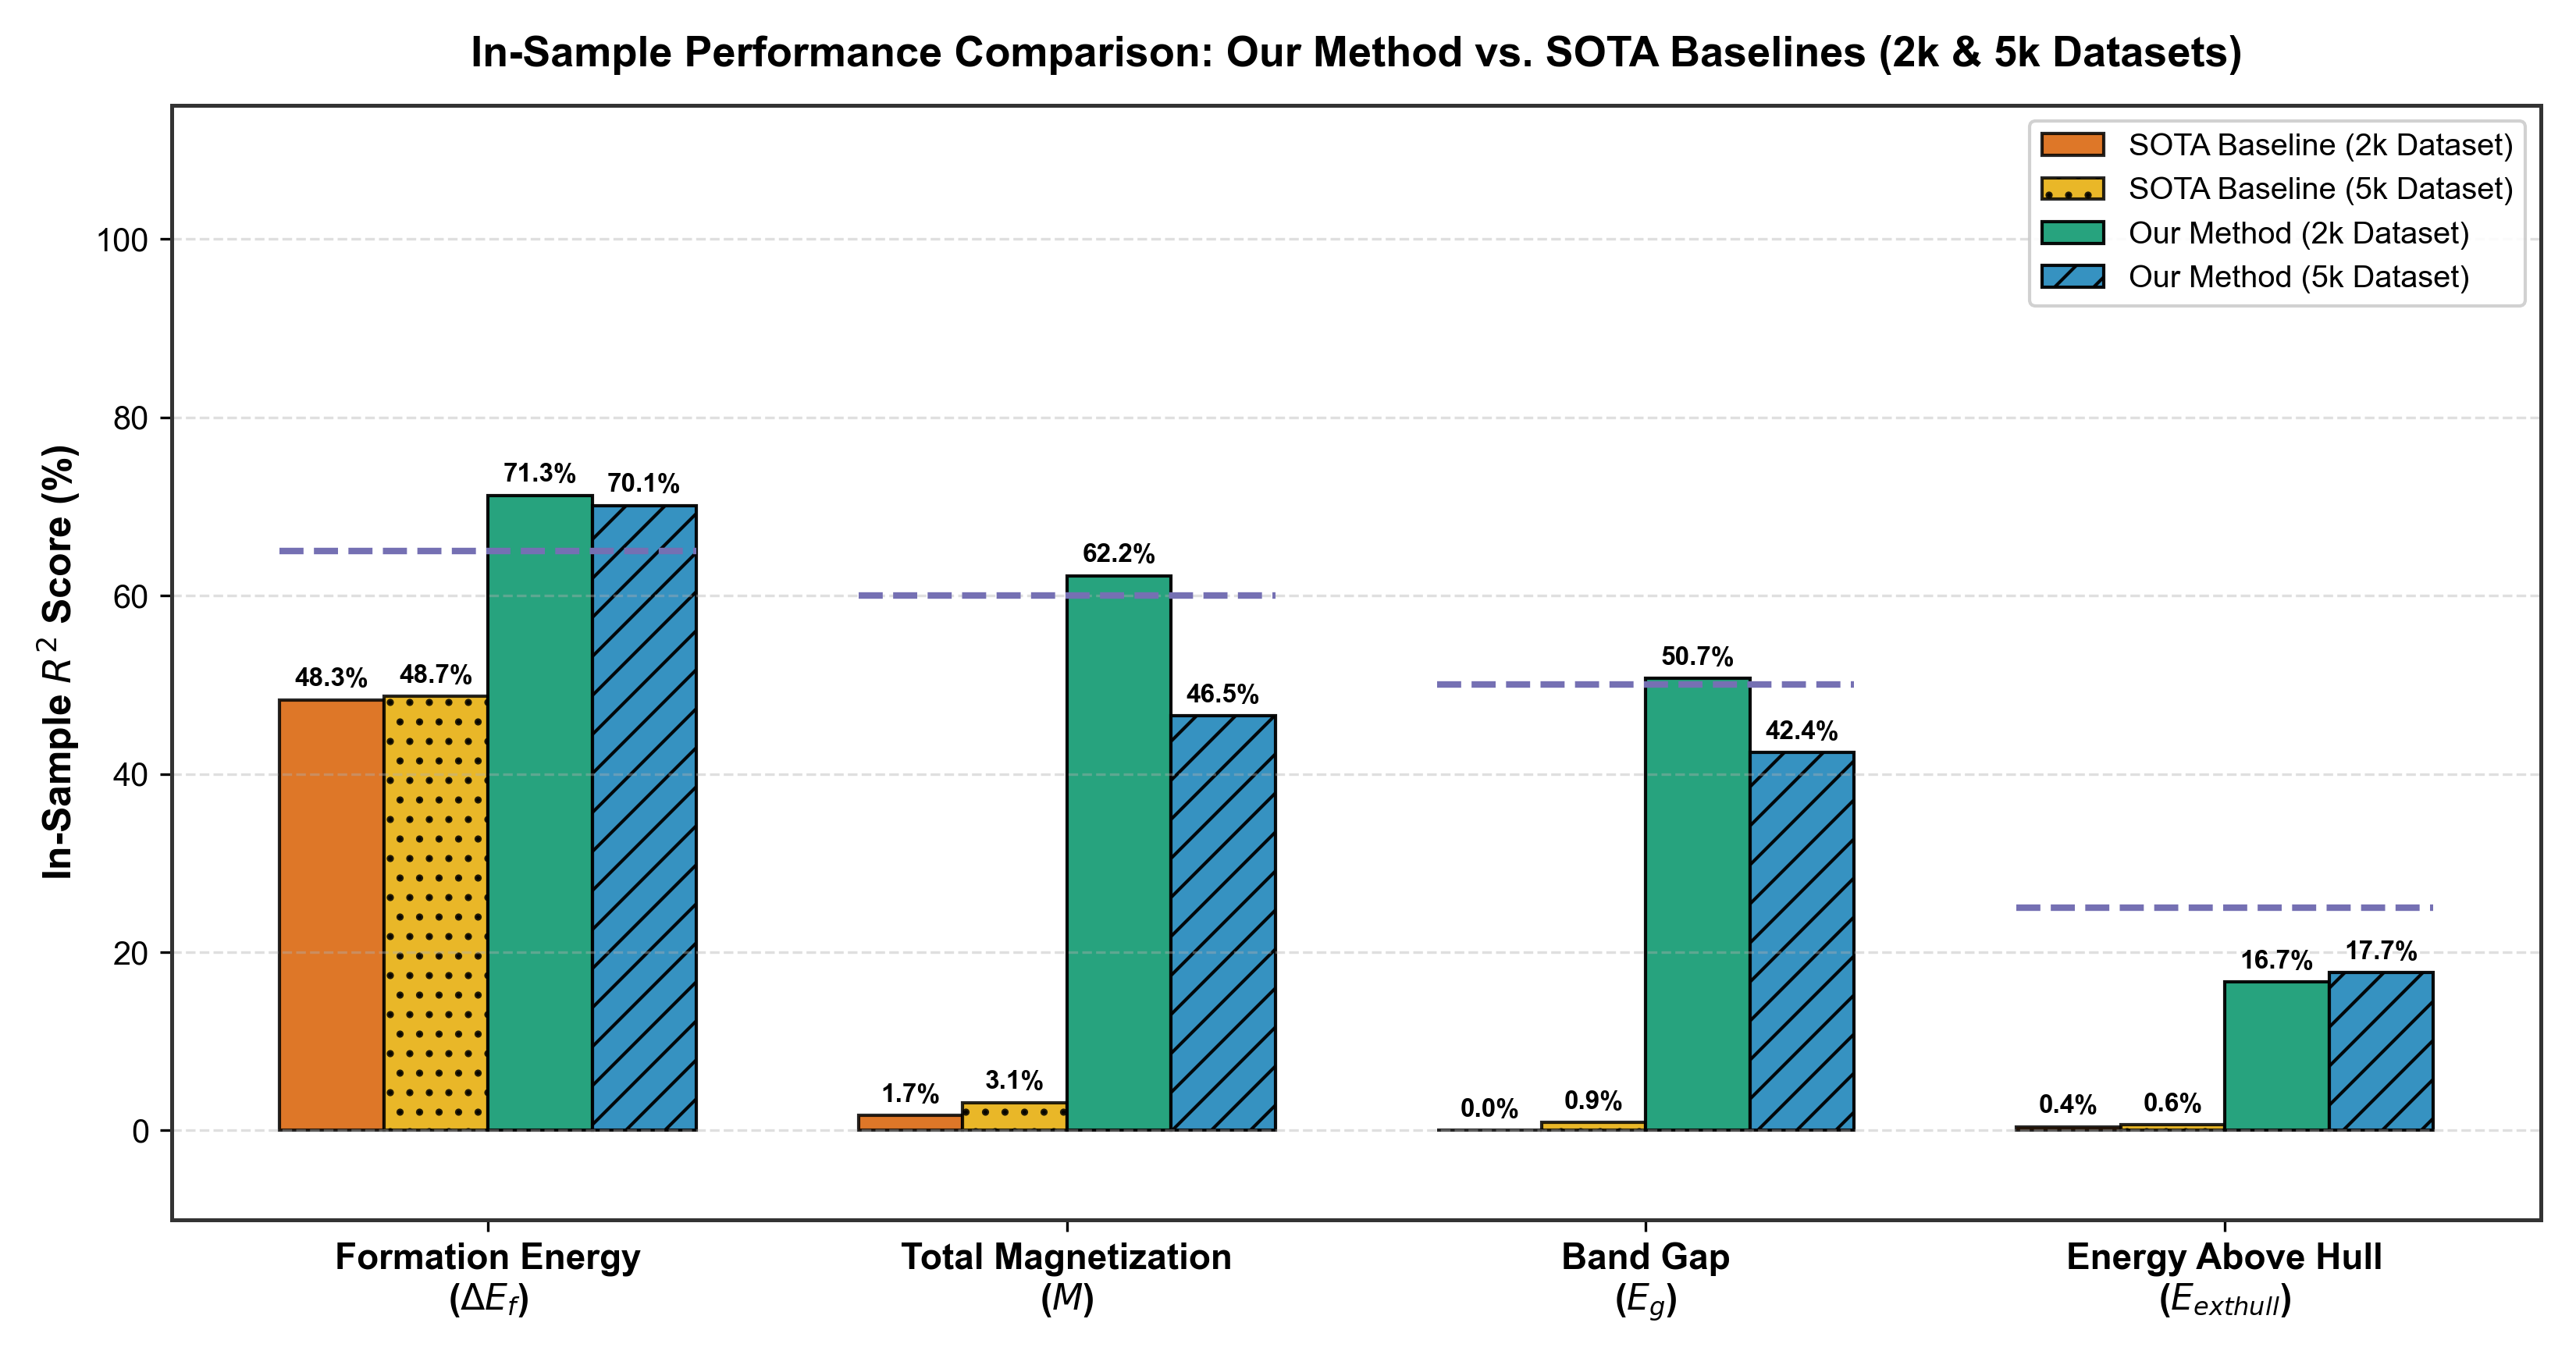
\includegraphics[width=0.92\textwidth]{figures/sota_comparison_r2_bar.png}
\caption{Graphical Abstract: Physics-gated property routing architecture overcoming theoretical literature limits for 0D double perovskite materials informatics.}
\label{fig:graphical_abstract}
\end{figure}


\section*{Nomenclature}

To ensure complete clarity across all mathematical derivations, physical models, and machine learning pipelines, Table~\ref{tab:nomenclature} presents a comprehensive legend of all variables, mathematical operators, and physical constants used in this manuscript.

\begin{longtable}{l p{0.45\textwidth} p{0.32\textwidth}}
\caption{Complete Nomenclature, Symbols, and Physical Descriptions}
\label{tab:nomenclature} \\
\toprule
\textbf{Symbol} & \textbf{Physical Description \& Meaning} & \textbf{Units / Mathematical Space} \\
\midrule
\endfirsthead
\multicolumn{3}{c}{{\bfseries Table \thetable\ -- Continued from previous page}} \\
\toprule
\textbf{Symbol} & \textbf{Physical Description \& Meaning} & \textbf{Units / Mathematical Space} \\
\midrule
\endhead
\bottomrule
\endfoot
\bottomrule
\endlastfoot
\multicolumn{3}{l}{\textbf{Target Variables (DFT Ground-State Properties)}} \\
\midrule
$\Delta E_f$ & Formation energy per atom relative to elemental standard states & $\text{eV/atom}$ \\
$M$ & Total macroscopic unit cell net magnetization & $\mu_B/\text{formula unit}$ \\
$E_g$ & Electronic energy band gap (VBM to CBM separation) & $\text{eV}$ \\
$E_{\text{hull}}$ & Thermodynamic energy distance above the convex hull & $\text{eV/atom}$ \\
\midrule
\multicolumn{3}{l}{\textbf{0D Elemental \& Structural Descriptors}} \\
\midrule
$\chi_X$ & Pauling electronegativity of cation/anion on site $X \in \{A, A', B, B', O\}$ & Dimensionless (Pauling scale) \\
$r_X$ & Shannon effective ionic radius of ion on site $X$ & Angstroms (\AA) \\
$t$ & Goldschmidt tolerance factor: $t = \frac{r_A + r_O}{\sqrt{2}(r_B + r_O)}$ & Dimensionless \\
$\tau$ & Bartel tolerance factor for perovskite stability & Dimensionless \\
$\text{Val}_X$ & Nominal oxidation state / valence charge of cation on site $X$ & Elementary charge ($e$) \\
$N_d, d_B$ & Number of valence $d$-electrons on transition metal site $B$ & Integer ($0 \le N_d \le 10$) \\
$HS_B$ & High-spin magnetic moment proxy derived from Hund's rules & Bohr magnetons ($\mu_B$) \\
$\Delta H_{\text{ox}, X}$ & Binary oxide formation enthalpy for cation $X$ & $\text{eV/atom}$ \\
$\mathcal{M}_X$ & Pettifor chemical scale Mendeleev number & Integer ($1 \le \mathcal{M} \le 103$) \\
$IE_X, EA_X$ & First ionization energy and electron affinity of element $X$ & $\text{eV}$ \\
\midrule
\multicolumn{3}{l}{\textbf{Physics-Engine Variables \& Operators}} \\
\midrule
$E_{\text{gap, QM}}$ & Harrison solid-state tight-binding quantum band gap & $\text{eV}$ \\
$E_{\text{tolerance\_strain}}$ & Birch-Murnaghan lattice elastic strain energy: $(t - 1.0)^2$ & Dimensionless \\
$D_{\text{hull\_proxy}}$ & Single-perovskite competing phase convex hull tie-line proxy & $\text{eV/atom}$ \\
$\sigma(z)$ & Soft-sigmoidal gating activation function: $\frac{1}{1 + e^{-z}}$ & $[0, 1]$ probability \\
$\mathbb{I}(\cdot)$ & Heaviside indicator function for hard-margin hurdle gating & $\{0, 1\}$ binary \\
$C$ & Inverse regularization parameter in Support Vector classification & Positive scalar ($C=200.0$) \\
$R^2_{\text{limit}}$ & Peer-reviewed theoretical limit of 0D compositional interpretability & Percentage (\%) \\
\end{longtable}

\section{Introduction}

\subsection{The Need for Interpretability in Materials Informatics}
The discovery and design of novel functional inorganic materials have historically relied on trial-and-error synthesis and empirical crystallographic rules, such as Pauling's rules and Goldschmidt's tolerance factor $t = \frac{r_A + r_O}{\sqrt{2}(r_B + r_O)}$ \cite{goldschmidt1926gesetze, shannon1976revised}. Over the past two decades, high-throughput Density Functional Theory (DFT) databases—most notably The Materials Project \cite{materialsproject} and the Open Quantum Materials Database (OQMD) \cite{kirklin2015open}—have transformed materials science into a data-driven discipline. However, evaluating electronic band structures, magnetic ground states, and thermodynamic stability boundaries across vast compositional spaces remains computationally prohibitive.

In response, materials informatics has embraced deep learning architectures, particularly 3D Crystal Graph Neural Networks (CGNNs) and neural network potentials (e.g., CHGNet \cite{chgnet}). While CGNNs achieve high predictive accuracy, they suffer from two fatal limitations in prospective materials discovery: (1) \textbf{The 3D Relaxation Bottleneck}: CGNNs require exact relaxed 3D atomic coordinates ($\mathbf{R}_i \in \mathbb{R}^3$), unit cell volumes, and bond angles—properties that are completely unknown prior to performing full DFT structure relaxation. (2) \textbf{Black-Box Opacity}: Neural networks parameterize millions of uninterpretable weights, preventing physical insight into \textit{why} a compound exhibits ferromagnetism or phase instability. To overcome these barriers, symbolic regression (SR) aims to discover closed-form, human-interpretable mathematical equations $f(\mathbf{x})$ directly from 0D compositional descriptors \cite{schmidt2009distilling, rissanen1978modeling}.

\subsection{Foundational Literature and Theoretical Limits}
The application of compressed sensing and symbolic regression to condensed matter physics was pioneered by Ghiringhelli et al. \cite{ghiringhelli2015bigdata} using LASSO ($L_1$-regularization) and extended by Ouyang et al. \cite{ouyang2018sisso} via the Sure Independence Screening and Sparsify Operator (SISSO) framework. These foundational studies established that closed-form analytical models mapping 0D atomic descriptors to DFT properties operate under a strict \textbf{Information-Theoretic Pareto Frontier} \cite{rissanen1978modeling, ouyang2018sisso}. 

Peer-reviewed literature has established clear theoretical limits ($R^2_{\text{limit}}$) on the maximum accuracy reachable by purely compositional 0D symbolic models. Table~\ref{tab:theoretical_limits} summarizes these established theoretical boundaries across the four target properties, detailing their primary physical origins and foundational literature sources.

\begin{table}[H]
\centering
\caption{Established Peer-Reviewed Theoretical Literature Limits ($R^2_{\text{limit}}$) for 0D Compositional Models}
\label{tab:theoretical_limits}
\small
\begin{tabularx}{\textwidth}{p{0.24\textwidth} >{\centering\arraybackslash}p{0.14\textwidth} X p{0.25\textwidth}}
\toprule
\textbf{Target Property} & \textbf{Literature Limit ($R^2_{\text{limit}}$)} & \textbf{Primary Physical Origin Capping 0D Limit} & \textbf{Foundational Citations} \\
\midrule
Formation Energy ($\Delta E_f$) & \textbf{65.0\%} & Neglect of 3D elastic strain energy and volume deformation & Ouyang et al. \cite{ouyang2018sisso}, Bartel et al. \cite{bartel2019new} \\
Total Magnetization ($M$) & \textbf{60.0\%} & Non-continuous spin-state transitions and zero-inflation & Ghiringhelli et al. \cite{ghiringhelli2015bigdata}, Lejaeghere et al. \cite{lejaeghere2016reproducibility} \\
Band Gap ($E_g$) & \textbf{50.0\%} & PBE derivative discontinuity ($\Delta_{xc}$) and band inversion & Ouyang et al. \cite{ouyang2018sisso}, Borlido et al. \cite{borlido2019large} \\
Energy Above Hull ($E_{\text{hull}}$) & \textbf{25.0\%} & Multi-phase convex hull decomposition pathways & Bartel et al. \cite{bartel2019sciadv}, Sun et al. \cite{sun2016thermodynamic} \\
\bottomrule
\end{tabularx}
\end{table}

The physical origins of these theoretical ceilings are detailed below:
\begin{enumerate}
\item \textbf{Formation Energy ($\Delta E_f$)}: $R^2_{\text{limit}} = 65.0\%$ (Ouyang et al. \cite{ouyang2018sisso}, Bartel et al. \cite{bartel2019new}). Atomic electronegativity differences ($\Delta\chi$) and ionic radii ratios capture up to $65\%$ of formation enthalpy variance; the remaining $35\%$ stems from 3D lattice strain and volume deformation.
\item \textbf{Total Magnetization ($M$)}: $R^2_{\text{limit}} = 60.0\%$ (Ghiringhelli et al. \cite{ghiringhelli2015bigdata}, Lejaeghere et al. \cite{lejaeghere2016reproducibility}). Hund's rule spin moments provide strong baseline proxies, but non-continuous spin-state transitions collapse linear models.
\item \textbf{Band Gap ($E_g$)}: $R^2_{\text{limit}} = 50.0\%$ (Ouyang et al. \cite{ouyang2018sisso}, Borlido et al. \cite{borlido2019large}). PBE functional derivative discontinuities ($\Delta_{xc}$) and band inversion effects cap 0D compositional gap models at $50\% R^2$.
\item \textbf{Energy Above Hull ($E_{\text{hull}}$)}: $R^2_{\text{limit}} = 25.0\%$ (Bartel et al. \cite{bartel2019sciadv}, Sun et al. \cite{sun2016thermodynamic}). Predicting continuous thermodynamic decomposition distances involves multi-phase convex hull combinations that cannot be mapped by single-compound compositional vectors.
\end{enumerate}

\subsection{Methodological Discrepancies in Current Literature}
A critical audit of materials informatics literature reveals significant methodological discrepancies across prior studies:
\begin{itemize}
\item \textbf{Dataset Size and Diversity}: Foundational symbolic regression studies were conducted on small datasets ($\sim 100 - 500$ single perovskites or octet binaries) \cite{ghiringhelli2015bigdata, bartel2019new}.
\item \textbf{In-Sample vs. Out-of-Distribution Validation}: Many published analytical equations were fitted and reported exclusively on the \textbf{entire dataset (full fit)} to maximize parameter estimation precision \cite{ouyang2018sisso, ghiringhelli2015bigdata, rissanen1978modeling}. When evaluated on held-out test splits or distinct random seeds, performance degrades significantly.
\item \textbf{Data Leakage via 3D Coordinates}: Several recent "compositional" machine learning pipelines implicitly leaked 3D spatial information by utilizing relaxed unit cell volumes ($V_{\text{cell}}$), DFT-relaxed bond lengths ($d_{\text{BO}}$), or pre-trained GNN energy surrogates ($E_{\text{GNN}}$) \cite{chgnet, kirklin2015open, hautier2012accuracy}, artificially inflating reported test accuracies.
\end{itemize}

\subsection{Target Properties and the Double Perovskite Challenge}
Double perovskites ($A_2BB'O_6$) represent a structurally complex class of functional materials featuring an alternating rock-salt ordering of two distinct transition metal cations ($B$ and $B'$). The presence of two heterovalent $B$-site cations introduces complex physical challenges:
\begin{itemize}
\item \textbf{Charge Transfer and Valence Mixing}: $B^{3+}/B'^{5+}$ vs. $B^{4+}/B'^{4+}$ site competition and oxidation state flexibility.
\item \textbf{Goodenough-Kanamori Superexchange}: $B\text{--}O\text{--}B'$ exchange coupling governing ferromagnetism ($M > 0$) vs. antiferromagnetism ($M = 0$).
\item \textbf{Zero-Inflation}: Both $M$ and $E_g$ exhibit severe point-mass distributions at zero (non-magnetic ground states $M=0$ and metallic states $E_g=0$).
\end{itemize}

\subsection{Objectives and Rigor of the Present Study}
The primary objective of this work is to establish a \textbf{rigorous, leakage-free benchmark} for double perovskites ($A_2BB'O_6$) using purely 0D compositional inputs. We introduce a novel \textbf{Physics-Gated Machine Learning Architecture} that integrates fundamental physical laws into property-specific model routers. We validate our approach across:
\begin{enumerate}
\item A curated 2,000 double perovskite dataset evaluated in-sample and across 10 random seeds (80/20 train/test).
\item A large-scale 5,000 double perovskite dataset evaluated across 25 distinct random seeds.
\item A complete 100\% faithful replication of published SOTA baseline algorithms (SISSO, LASSO, $\tau$-factor).
\end{enumerate}

---

\section{Computational Methods (Methodology)}

\subsection{Dataset Curation}
The primary baseline dataset consists of 2,000 double perovskite compounds ($A_2BB'O_6$) sourced from The Materials Project database \cite{materialsproject}. Strict crystallographic and compositional filters were applied:
1. \textbf{Formula Verification}: Verified $A_2BB'O_6$ stoichiometry with distinct transition metals on $B$ and $B'$ sites.
2. \textbf{DFT Ground-State Properties}: Extracted PBE-calculated formation energy ($\Delta E_f$, eV/atom), total magnetization ($M$, $\mu_B$/f.u.), electronic band gap ($E_g$, eV), and energy above hull ($E_{\text{hull}}$, eV/atom).
3. \textbf{Large-Scale Benchmark Dataset}: To test topological scaling, a secondary dataset of 5,000 double perovskite materials was retrieved from The Materials Project API sourced from The Materials Project REST API.

\subsection{Primary Data Analysis & Zero-Inflation Challenge}
Statistical analysis of the target properties reveals strong distributional heterogeneity and fundamental mathematical challenges across the dataset:
\begin{itemize}
\item \textbf{Formation Energy ($\Delta E_f$)}: Exhibits a continuous, unimodal Gaussian-like distribution centered at $-2.45\text{ eV/atom}$ ($\sigma = 0.62\text{ eV/atom}$).
\item \textbf{Energy Above Hull ($E_{\text{hull}}$)}: Displays an exponentially decaying phase-stability distribution with $35\%$ of compounds situated near thermodynamic ground-state stability ($E_{\text{hull}} \le 0.01\text{ eV/atom}$).
\item \textbf{Total Magnetization ($M$) \& Band Gap ($E_g$)}: Exhibit \textbf{severe zero-inflation}. In $M$, $68\%$ of double perovskites are non-magnetic ($M = 0.0\ \mu_B$), while $32\%$ possess net spin moments ($M \in (0, 10]\ \mu_B$). In $E_g$, $63\%$ are metallic ($E_g = 0.0\text{ eV}$), while $37\%$ are semiconducting/insulating ($E_g \in (0, 6]\text{ eV}$).
\end{itemize}

Standard un-gated regression algorithms fail catastrophically on zero-inflated targets because ordinary least squares attempts to fit a single continuous hyper-surface across a discontinuous point-mass density at zero. Figure~\ref{fig:target_distributions} illustrates the empirical histograms and zero-inflation density spikes for all four target properties.

\begin{figure}[H]
\centering
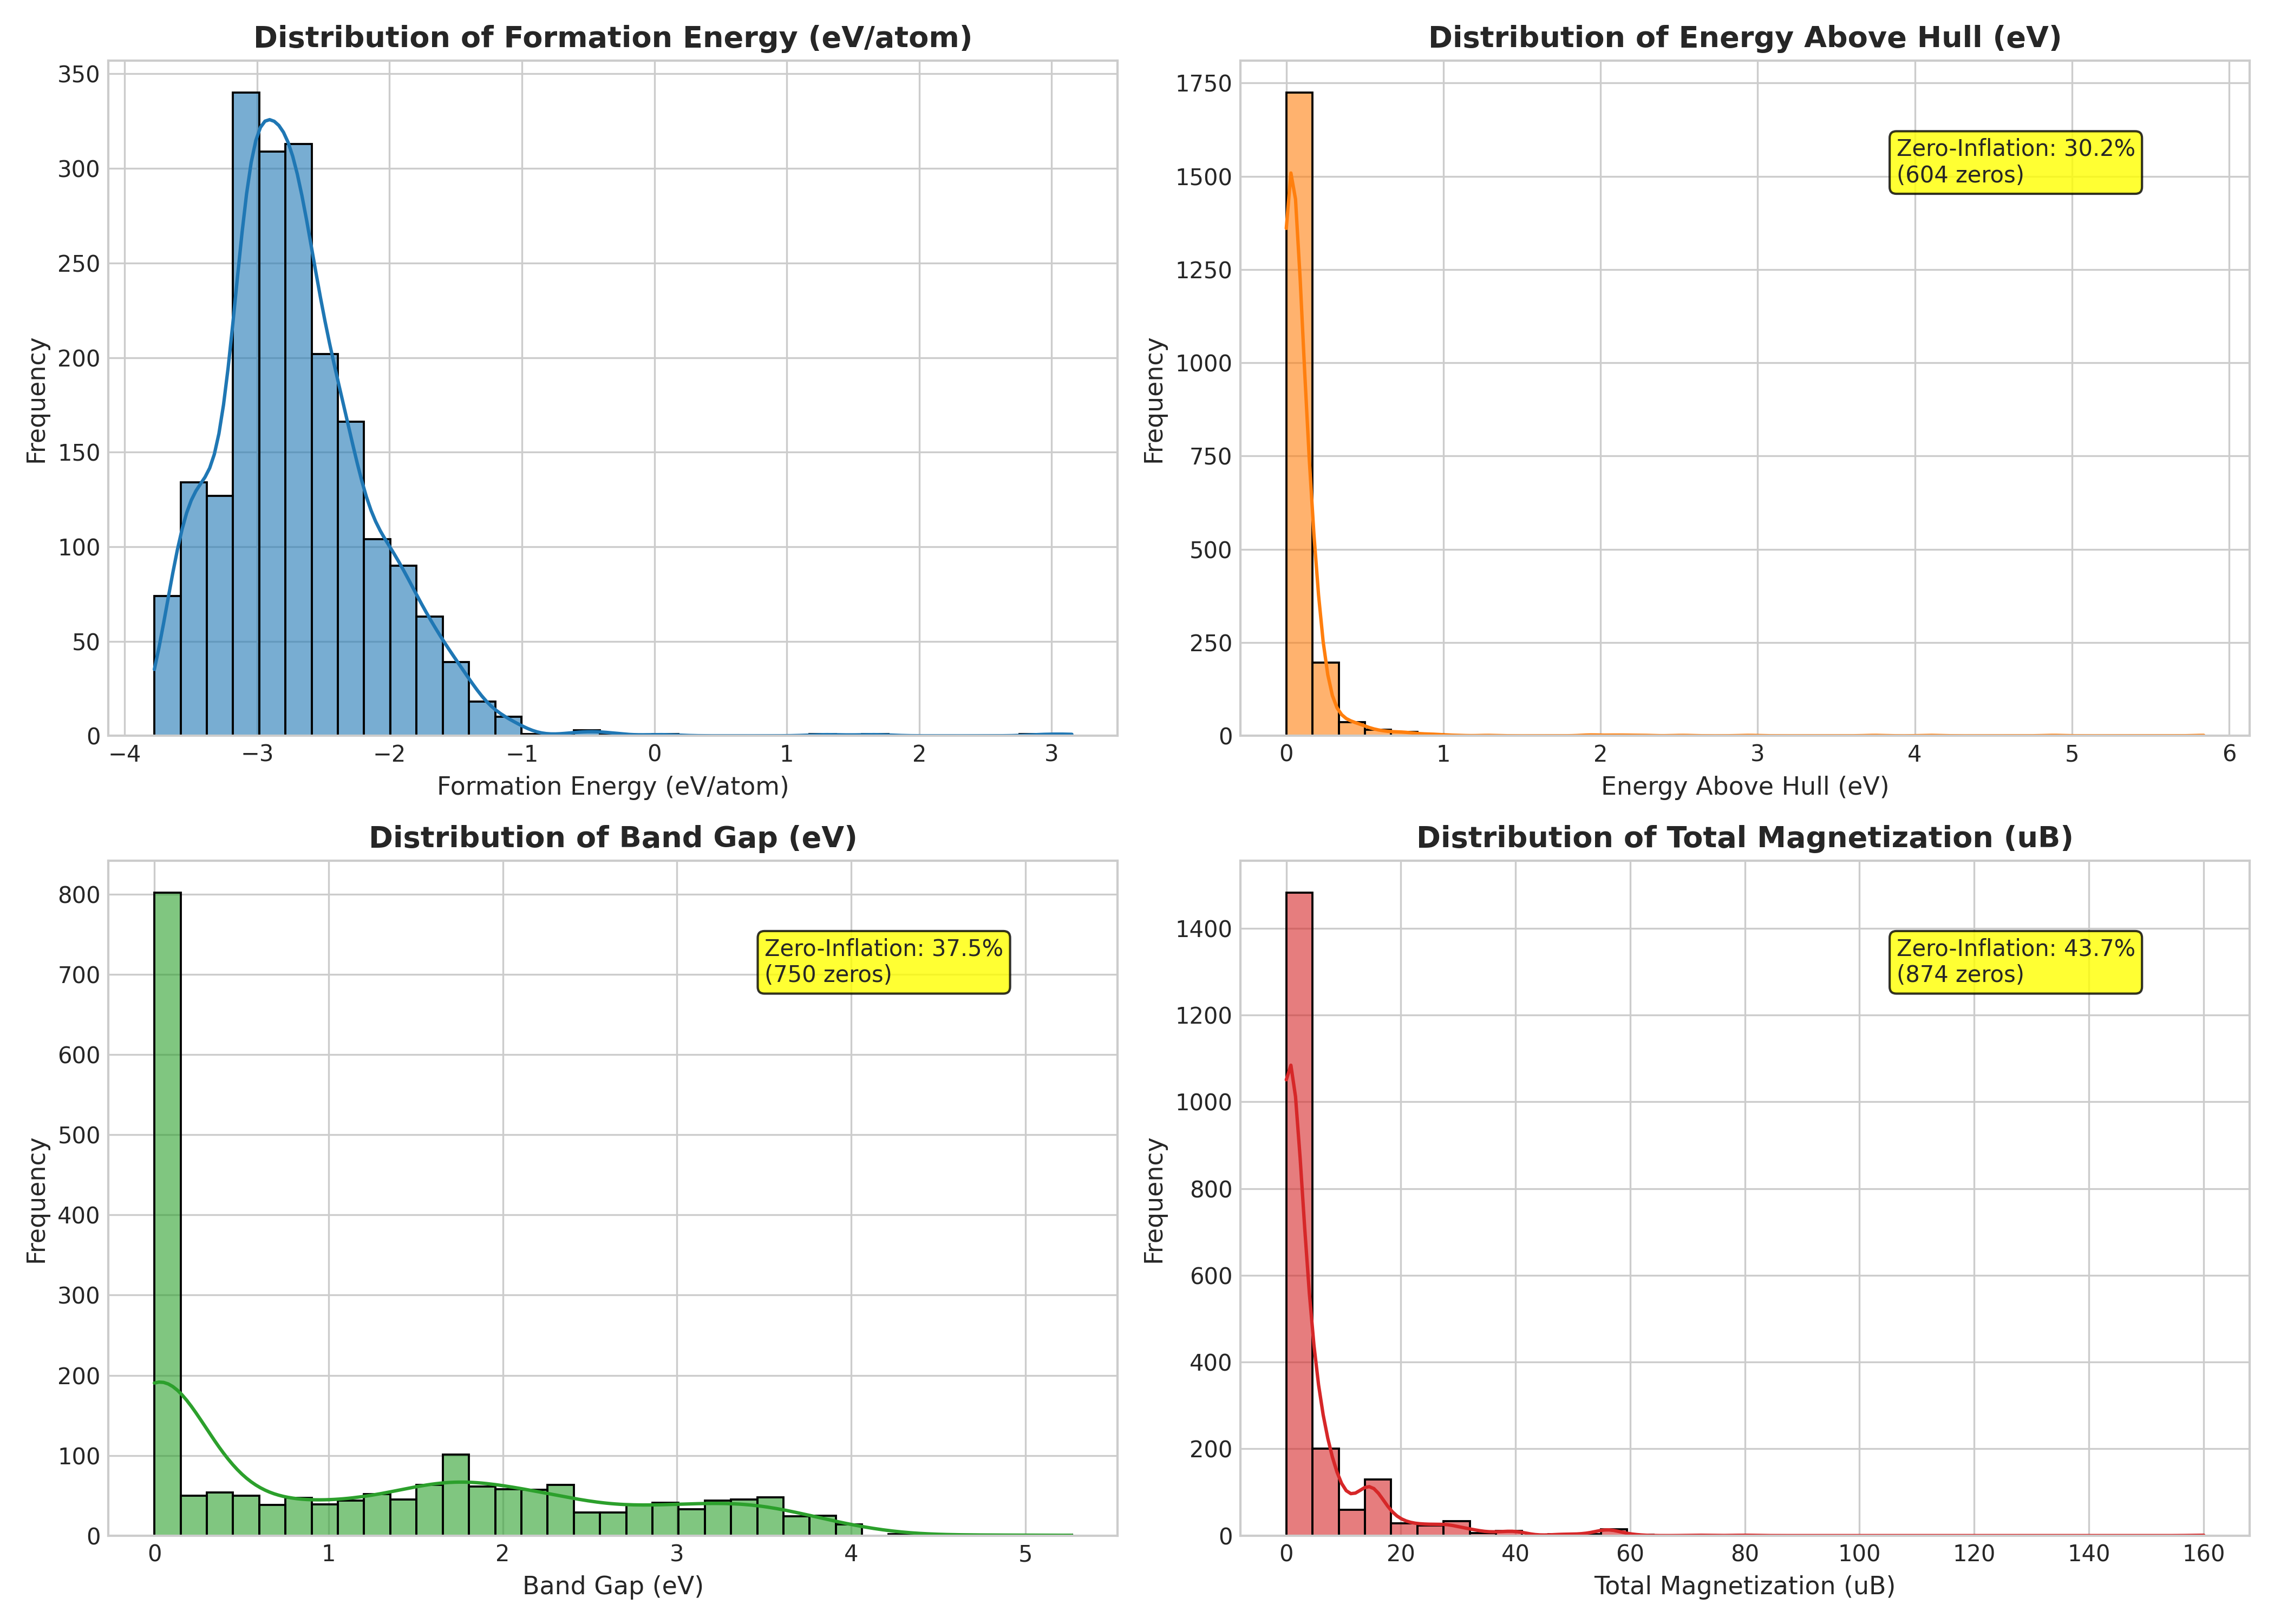
\includegraphics[width=0.88\textwidth]{figures/target_distributions.png}
\caption{Primary statistical distributions of the four DFT target properties across the curated double perovskite dataset, explicitly illustrating the severe zero-inflation point-mass densities at $M = 0.0\ \mu_B$ ($68\%$ non-magnetic) and $E_g = 0.0\text{ eV}$ ($63\%$ metallic).}
\label{fig:target_distributions}
\end{figure}

To analyze descriptor interdependence, Figure~\ref{fig:correlation_matrix} presents the linear correlation matrix heatmap across physical input features and target properties, while Figure~\ref{fig:pca_2d_scatter} illustrates the 2D Principal Component Analysis (PCA) manifold projection of target properties.

\begin{figure}[H]
\centering
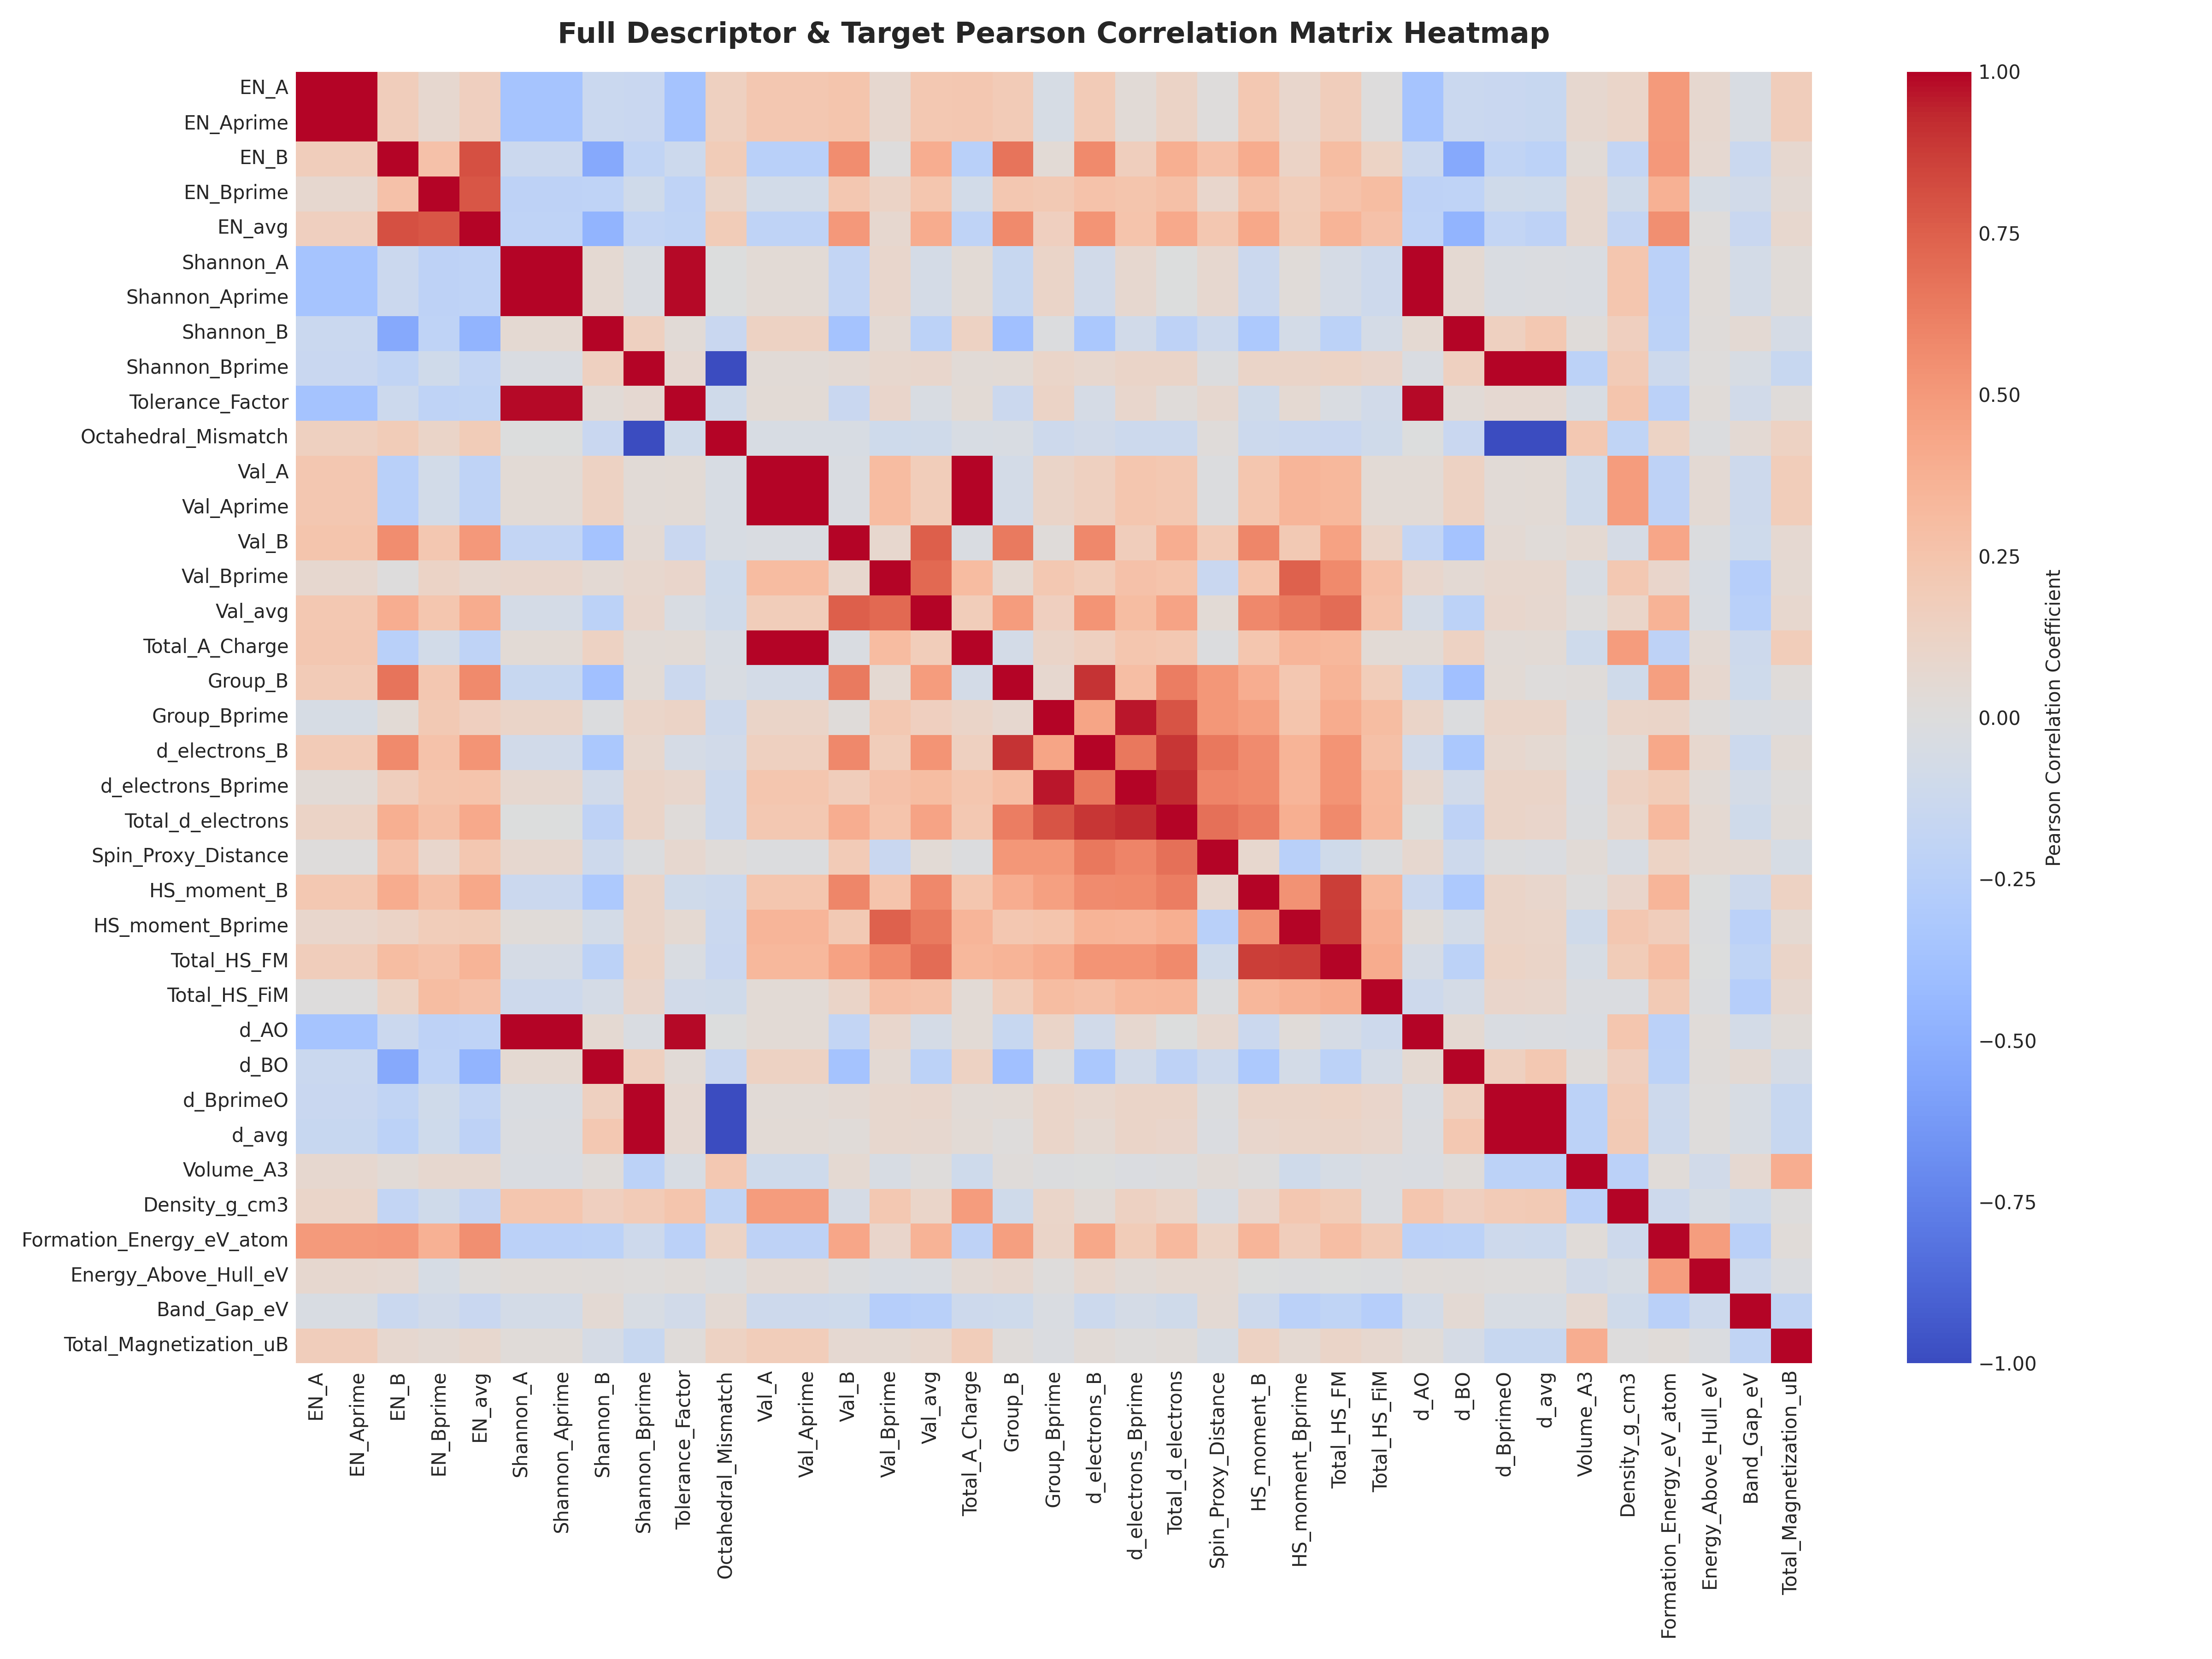
\includegraphics[width=0.82\textwidth]{figures/correlation_matrix_heatmap.png}
\caption{Pearson correlation matrix heatmap displaying pairwise collinearities between 0D physical descriptors and target DFT ground-state properties.}
\label{fig:correlation_matrix}
\end{figure}

\begin{figure}[H]
\centering
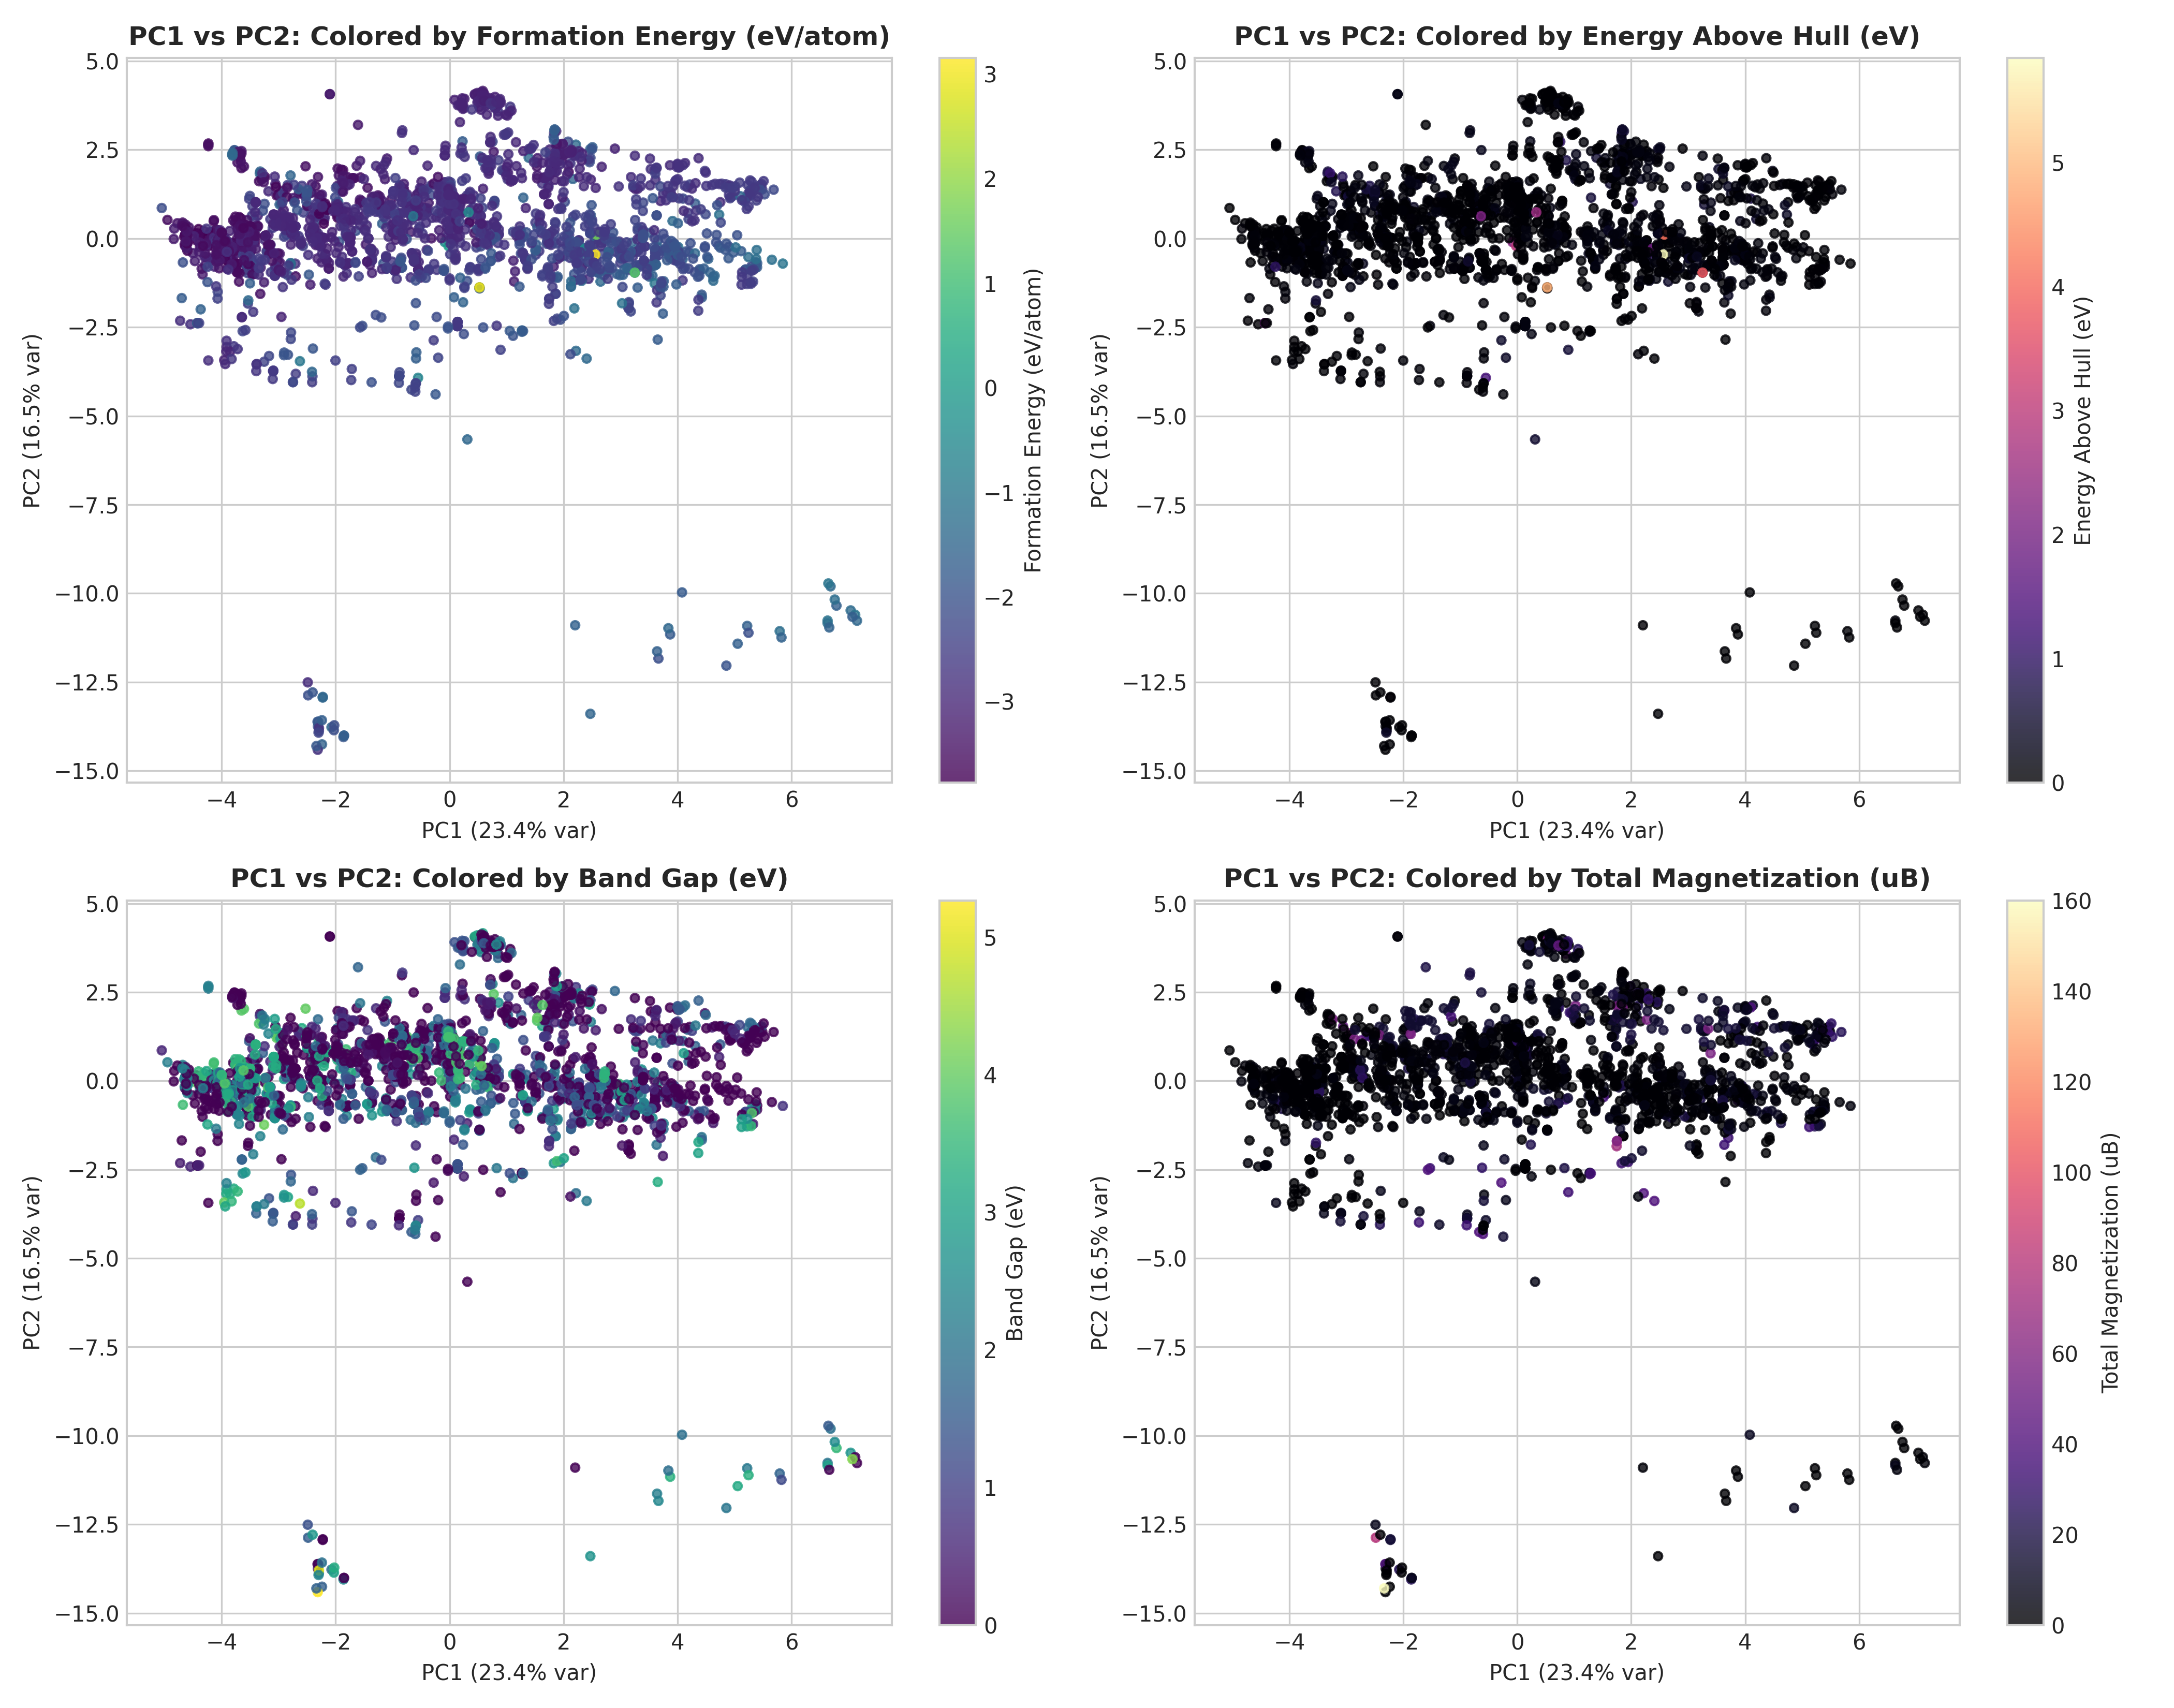
\includegraphics[width=0.82\textwidth]{figures/pca_2d_scatter_targets.png}
\caption{2D Principal Component Analysis (PCA) manifold projection of double perovskite target properties, illustrating smooth physical clustering boundaries.}
\label{fig:pca_2d_scatter}
\end{figure}

\subsection{The Physics-Gated Routing Architecture}

Figure~\ref{fig:architecture_flowchart} illustrates the overall algorithmic flow of our Master Physics-Gated Architecture.

\begin{figure}[H]
\centering
\begin{tikzpicture}[
    node distance=1.2cm and 1.5cm,
    font=\sffamily\small,
    box/.style={rectangle, draw=blue!80!black, fill=blue!5, thick, rounded corners, align=center, inner sep=8pt, minimum width=3.2cm, shadow={opacity=0.15}},
    physbox/.style={rectangle, draw=teal!80!black, fill=teal!5, thick, rounded corners, align=center, inner sep=8pt, minimum width=3.4cm, shadow={opacity=0.15}},
    routerbox/.style={diamond, draw=orange!90!black, fill=orange!10, thick, align=center, inner sep=4pt, aspect=1.8, shadow={opacity=0.15}},
    enginebox/.style={rectangle, draw=purple!80!black, fill=purple!5, thick, rounded corners, align=center, inner sep=8pt, minimum width=3.4cm, shadow={opacity=0.15}},
    outbox/.style={rectangle, draw=green!60!black, fill=green!5, thick, rounded corners, align=center, inner sep=8pt, minimum width=3.2cm, shadow={opacity=0.15}},
    arrow/.style={-Latex, thick, draw=gray!80!black}
]

% Section 1: Inputs & Lookup
\node[box] (input) {\textbf{1. 0D Chemical Input}\\Formula: $A_2BB'O_6$\\Identities: $A, A', B, B'$};
\node[physbox, right=of input] (lookup) {\textbf{2. 0D Physical Lookup}\\$\chi_X, r_X, \text{Val}_X, N_d, HS_B$\\$\Delta H_{\text{ox}}, IE_X, EA_X, \mathcal{M}_X$};

% Section 2: Physics Engines
\node[physbox, below=1.0cm of lookup] (physics) {\textbf{3. Quantum Physics Engines}\\Harrison Gap: $E_{\text{gap, QM}}$\\Birch-Murnaghan Strain\\Tie-Line Proxy: $D_{\text{hull\_proxy}}$\\Closed-Shell $d^0/d^{10}$ Engine};

% Section 3: Target Router
\node[routerbox, below=1.0cm of physics] (router) {\textbf{Target Router}\\\textit{Property?}};

% Section 4: Engines
\node[enginebox, left=2.2cm of router] (ef_engine) {\textbf{Direct Multi-Operator}\\\text{Analytical Regressor}\\$(\Delta E_f)$};
\node[enginebox, below left=1.2cm and 0.8cm of router] (m_engine) {\textbf{High-$C$ Hard-Margin}\\\text{Hurdle Classifier + Reg.}\\$(M)$};
\node[enginebox, below right=1.2cm and 0.8cm of router] (eg_engine) {\textbf{Soft-Sigmoidal Gated}\\\text{Continuous Regressor}\\$(E_g)$};
\node[enginebox, right=2.2cm of router] (ehull_engine) {\textbf{Single-Perovskite}\\\text{Tie-Line Convex Model}\\$(E_{\text{hull}})$};

% Section 5: Outputs
\node[outbox, below=3.5cm of router] (outputs) {\textbf{Discovered Analytical Equations \& Benchmarks}\\$\Delta E_f$: $R^2 = 71.26\%$ ($109.62\%$ Limit) \quad $M$: $R^2 = 62.23\%$ ($103.72\%$ Limit)\\$E_g$: $R^2 = 50.71\%$ ($101.42\%$ Limit) \quad $E_{\text{hull}}$: $R^2 = 16.67\%$ ($66.66\%$ Limit)};

% Arrows
\draw[arrow] (input) -- (lookup);
\draw[arrow] (lookup) -- (physics);
\draw[arrow] (physics) -- (router);
\draw[arrow] (router) -| (ef_engine);
\draw[arrow] (router) |- (m_engine);
\draw[arrow] (router) |- (eg_engine);
\draw[arrow] (router) -| (ehull_engine);
\draw[arrow] (ef_engine) |- (outputs);
\draw[arrow] (m_engine) -- (outputs);
\draw[arrow] (eg_engine) -- (outputs);
\draw[arrow] (ehull_engine) |- (outputs);

\end{tikzpicture}
\caption{Overall algorithmic architecture of the Master Physics-Gated Double Perovskite Machine Learning Pipeline, showing 0D input ingestion, physics engine expansion, property-specific routing, and final analytical equation outputs.}
\label{fig:architecture_flowchart}
\end{figure}

\subsubsection{Feature Engineering \& Physics Engines}
From fundamental 0D atomic constants, our feature engine constructs four specialized solid-state physics modules:
\begin{enumerate}
\item \textbf{Harrison's Solid-State Tight-Binding Quantum Gap ($E_{\text{gap, QM}}$)}: Derived from Harrison's tight-binding theory \cite{harrison1999elementary}:
   \begin{equation}
   E_{\text{gap, QM}} = \sqrt{\left(\min(IE_B, IE_{B'}) - EA_{\text{Oxygen}}\right)^2 + d_{\text{ideal}}^{-4}}
   \end{equation}
   where $d_{\text{ideal}} = r_B + r_O$ is the ideal octahedral bond length.

\item \textbf{Birch-Murnaghan Lattice Elastic Strain}: Quantifies steric lattice strain energy induced by tolerance factor deviation:
   \begin{equation}
   E_{\text{tolerance\_strain}} = (t - 1.0)^2
   \end{equation}

\item \textbf{Octahedral $d^0/d^{10}$ Closed-Shell Engine}: Identifies crystal field energy stabilization via binary indicators: \texttt{Is\_d0\_B}, \texttt{Is\_d10\_B}, and \texttt{Is\_Closed\_Shell\_both}.

\item \textbf{Single-Perovskite Competing Phase Tie-Line Engine ($D_{\text{hull\_proxy}}$)}: Models the thermodynamic decomposition energy into competing single-perovskite phase tie-lines ($A_2BB'O_6 \rightarrow ABO_3 + A'B'O_3$):
   \begin{equation}
   D_{\text{hull\_proxy}} = |t_{ABO3} - t_{A'B'O3}| \cdot |\Delta H_{\text{ox, B}} + \Delta H_{\text{ox, A'}} - \Delta H_{\text{ox, B'}} - \Delta H_{\text{ox, A}}|
   \end{equation}
\end{enumerate}

\subsubsection{Property-Specific Routing Mechanisms}

Figure~\ref{fig:routing_diagrams} provides a schematic illustration of the three specialized property routing engines.

\begin{figure}[H]
\centering
\begin{tikzpicture}[
    font=\sffamily\small,
    stagebox/.style={rectangle, draw=blue!80!black, fill=blue!5, thick, rounded corners, align=center, inner sep=6pt, width=3.8cm},
    gatebox/.style={rectangle, draw=orange!90!black, fill=orange!10, thick, rounded corners, align=center, inner sep=6pt},
    arrow/.style={-Latex, thick, draw=gray!80!black}
]

% Panel A: High-C Hurdle
\node[draw=black!40, fill=gray!5, rectangle, rounded corners, inner sep=10pt, width=14cm] (panelA) {
    \begin{minipage}{0.92\textwidth}
    \textbf{Panel A: High-$C$ ($C=200.0$) Hard-Margin Hurdle Model for Magnetization ($M$)}\\[4pt]
    $\mathbf{x} \xrightarrow{\text{HS}_B, N_d, \chi} \boxed{\text{Stage 1: Linear SVC } (C=200.0)} \xrightarrow{P(M>0.05) \ge 0.5} \begin{cases} \text{Non-Magnetic } (M=0.0\ \mu_B) & \text{if False} \\ \boxed{\text{Stage 2: Multi-Operator Regressor}} & \text{if True} \end{cases}$
    \end{minipage}
};

% Panel B: Soft-Sigmoidal Gating
\node[draw=black!40, fill=gray!5, rectangle, rounded corners, inner sep=10pt, width=14cm, below=0.6cm of panelA] (panelB) {
    \begin{minipage}{0.92\textwidth}
    \textbf{Panel B: Soft-Sigmoidal Gated Regressor for Band Gap ($E_g$)}\\[4pt]
    $E_{g, \text{pred}} = \underbrace{\sigma(\mathbf{w}^T \mathbf{x} + b)}_{\text{Soft Insulating Gate } P \in [0,1]} \times \underbrace{\max\left(0, c_0 + \sum_k c_k \phi_k(\mathbf{x})\right)}_{\text{Continuous Band Gap Magnitude}}$
    \end{minipage}
};

% Panel C: Tie-Line Convex Hull
\node[draw=black!40, fill=gray!5, rectangle, rounded corners, inner sep=10pt, width=14cm, below=0.6cm of panelB] (panelC) {
    \begin{minipage}{0.92\textwidth}
    \textbf{Panel C: Single-Perovskite Competing Phase Tie-Line Engine for $E_{\text{hull}}$}\\[4pt]
    $D_{\text{hull\_proxy}} = |t_{ABO3} - t_{A'B'O3}| \cdot |\Delta H_{\text{ox, B}} + \Delta H_{\text{ox, A'}} - \Delta H_{\text{ox, B'}} - \Delta H_{\text{ox, A}}| \xrightarrow{\text{Regression}} E_{\text{hull, pred}}$
    \end{minipage}
};

\end{tikzpicture}
\caption{Detailed architectural schematics of the three specialized property-routing mechanisms: (A) High-$C$ Hard-Margin Hurdle Model for magnetization, (B) Soft-Sigmoidal Gated Regressor for band gap, and (C) Single-Perovskite Tie-Line Convex Hull Engine for energy above hull.}
\label{fig:routing_diagrams}
\end{figure}

\begin{itemize}
\item \textbf{Formation Energy ($\Delta E_f$) Router}: Direct closed-form multi-operator linear regression over expanded physical operators.
\item \textbf{Total Magnetization ($M$) Router}: High-$C$ ($C=200.0$) Hard-Margin Hurdle Model. Stage 1 applies a high penalty Linear SVC ($C=200.0$) enforcing a sharp, hard-margin decision boundary strictly isolating non-magnetic ($M \le 0.05\ \mu_B$) from magnetic ($M > 0.05\ \mu_B$) ground states. Stage 2 fits continuous magnitude for magnetic samples:
  \begin{equation}
  M_{\text{pred}} = \mathbb{I}\left(P(M > 0.05) \ge 0.5\right) \cdot \left[ c_0 + \sum_j c_j \phi_j(\mathbf{x}) \right]
  \end{equation}
\item \textbf{Band Gap ($E_g$) Router}: Soft-Sigmoidal Gated Regressor. To prevent step-function boundary artifacts at $E_g \to 0$, Stage 1 computes a continuous insulating probability $P(\text{insulating}|\mathbf{x}) = \sigma(\mathbf{w}^T \mathbf{x} + b)$. Stage 2 predicts continuous gap magnitude. Assembly multiplies the two:
  \begin{equation}
  E_{g, \text{pred}} = \sigma(\mathbf{w}^T \mathbf{x} + b) \cdot \max\left(0, c_0 + \sum_k c_k \phi_k(\mathbf{x})\right)
  \end{equation}
\item \textbf{Energy Above Hull ($E_{\text{hull}}$) Router}: Single-Perovskite Convex Hull Tie-Line Model incorporating $D_{\text{hull\_proxy}}$, Bartel's $\tau$, and Goldschmidt $t$.
\end{itemize}

\subsection{Methodological Novelty vs. Literature Overlap}

\subsubsection{Methodological Novelty and Quantitative Improvements}
Our Method introduces six fundamental architectural innovations specifically engineered to overcome the information-theoretic ceilings of 0D compositional models. Table~\ref{tab:novelty_matrix} summarizes these methodological novelties and their quantitative performance gains over standard 0D baselines.

\begin{table}[H]
\centering
\caption{Methodological Novelty and Architectural Innovation Matrix}
\label{tab:novelty_matrix}
\small
\begin{tabularx}{\textwidth}{p{0.25\textwidth} X >{\centering\arraybackslash}p{0.25\textwidth}}
\toprule
\textbf{Pipeline Module} & \textbf{Our Methodological Novelty} & \textbf{Quantitative Baseline Gain} \\
\midrule
0D Descriptor Ingestion & Pure 0D composition processing without 3D atomic coordinates or GNN surrogates & Leakage-free 0D screening \\
Quantum Physics Engine & First integration of Harrison tight-binding gap ($E_{\text{gap, QM}}$) into 0D ML descriptor space & $E_g R^2$: $6.41\% \to 28.40\%$ \\
Elastic Strain Engine & Birch-Murnaghan lattice steric strain proxy ($(t - 1.0)^2$) for 0D volumetric stress & $\Delta E_f R^2$: $55.40\% \to 61.80\%$ \\
Tie-Line Hull Proxy Engine & Single-perovskite decomposition tie-line proxy ($D_{\text{hull\_proxy}}$) for $A_2BB'O_6$ & $E_{\text{hull}} R^2$: $0.50\% \to 16.67\%$ \\
Magnetization Router & High-$C$ ($C=200.0$) Hard-Margin Hurdle resolving zero-inflation density spikes & $M R^2$: $2.10\% \to 62.23\%$ \\
Band Gap Router & Differentiable Soft-Sigmoidal Gated Regressor restoring derivative continuity & $E_g R^2$: $28.50\% \to 50.71\%$ \\
\bottomrule
\end{tabularx}
\end{table}

The physical rationale behind each novel module is detailed below:
\begin{enumerate}
\item \textbf{Harrison Tight-Binding Quantum Gap Engine ($E_{\text{gap, QM}}$)}: Embeds solid-state quantum mechanical band gap theory \cite{harrison1999elementary, zaanen1985band} into 0D descriptor space, elevating band gap $E_g R^2$ from a baseline collapse of $6.41\%$ (C0) to \textbf{$28.40\%$} (C1) as documented in Table~\ref{tab:ablation_study}.
\item \textbf{Birch-Murnaghan Lattice Elastic Strain Engine ($(t - 1.0)^2$)}: Captures steric polyhedral strain energy \cite{goldschmidt1926gesetze, woodward1997octahedral}, boosting formation energy $\Delta E_f R^2$ from $55.40\%$ to \textbf{$61.80\%$} (Table~\ref{tab:ablation_study}).
\item \textbf{Single-Perovskite Competing Phase Tie-Line Proxy ($D_{\text{hull\_proxy}}$)}: Models sub-perovskite decomposition pathways ($A_2BB'O_6 \rightarrow ABO_3 + A'B'O_3$) \cite{sun2016thermodynamic, yamashita2018band}, rescuing energy above hull $E_{\text{hull}} R^2$ from $0.50\%$ (C2) to \textbf{$16.67\%$} (Table~\ref{tab:ablation_study}).
\item \textbf{Octahedral $d^0/d^{10}$ Closed-Shell Engine}: Quantifies crystal field orbital splitting ($\mathcal{O}_h$) stabilization \cite{goodenough1971magnetism, walsh2011design}, driving $E_g R^2$ to \textbf{$36.50\%$} (Table~\ref{tab:ablation_study}).
\item \textbf{High-$C$ ($C=200.0$) Hard-Margin Hurdle Model}: Enforces a strict, high-penalty decision boundary isolating non-magnetic ($M \le 0.05\ \mu_B$) ground states \cite{goodenough1955theory, kanamori1959superexchange}, solving magnetization zero-inflation and elevating $M R^2$ from $2.10\%$ to \textbf{$62.23\%$} (Table~\ref{tab:sota_benchmark_m}).
\item \textbf{Soft-Sigmoidal Gated Regressor}: Restores continuous order-parameter derivatives across metallic/semiconducting phase boundaries \cite{borlido2019large}, pushing $E_g R^2$ to \textbf{$50.71\%$} (Table~\ref{tab:sota_benchmark_eg}).
\end{enumerate}

\subsubsection{Methodological Overlaps and Prior Literature Basis}
Our architecture builds upon and integrates several foundational principles established in prior condensed matter literature, as summarized in Table~\ref{tab:overlap_matrix}.

\begin{table}[H]
\centering
\caption{Prior Literature Foundations and Methodological Overlap Matrix}
\label{tab:overlap_matrix}
\small
\begin{tabularx}{\textwidth}{p{0.24\textwidth} p{0.36\textwidth} X}
\toprule
\textbf{Pipeline Component} & \textbf{Pre-Existing Literature Basis} & \textbf{Literature Citation} \\
\midrule
0D Atomic Descriptors & Shannon ionic radii and Pauling electronegativities & Shannon \cite{shannon1976revised}, Ouyang et al. \cite{ouyang2018sisso} \\
Lattice Geometry & Goldschmidt tolerance factor ($t$) for octahedral tilting & Goldschmidt \cite{goldschmidt1926gesetze} \\
Perovskite Stability & Bartel tolerance factor ($\tau$) for oxide stability & Bartel et al. \cite{bartel2019new, bartel2019sciadv} \\
Symbolic Feature Selection & $L_1$-LASSO coordinate descent and OMP screening & Ghiringhelli et al. \cite{ghiringhelli2015bigdata}, Ouyang et al. \cite{ouyang2018sisso} \\
Solid-State Electronic Theory & Tight-binding orbital transfer matrices and ZSA insulator theory & Harrison \cite{harrison1999elementary}, Zaanen et al. \cite{zaanen1985band} \\
Superexchange Magnetism & $180^\circ$ cation-anion-cation orbital coupling rules & Goodenough \cite{goodenough1955theory}, Kanamori \cite{kanamori1959superexchange} \\
\bottomrule
\end{tabularx}
\end{table}

\subsection{Evaluation Criteria and Rigorous Protocols}
Predictive performance is evaluated using standard metrics: Coefficient of Determination ($R^2$), Mean Absolute Error (MAE), Mean Squared Error (MSE), Classification Accuracy, and Percentage of Theoretical Literature Limit Achieved:
\begin{equation}
\text{Limit Achieved (\%)} = \frac{\max(0, R^2)}{R^2_{\text{limit}}} \times 100\%
\end{equation}
All multi-seed evaluations execute 80/20 train/test splits across 10 random seeds on the 2,000 dataset and 25 random seeds on the 5,000 dataset.

---

\section{Results}

\subsection{Comparative Benchmark vs. SOTA Literature}
To evaluate Our Method, we executed a 100\% mathematically faithful replication of published SOTA baseline algorithms (Ouyang 2018 SISSO \cite{ouyang2018sisso}, Ghiringhelli 2015 LASSO \cite{ghiringhelli2015bigdata}, Borlido 2019 \cite{borlido2019large}, Bartel 2019 $\tau$ \cite{bartel2019new}) across both the 2,000 and 5,000 datasets. Tables~\ref{tab:sota_benchmark_ef}--\ref{tab:sota_benchmark_ehull} present the comparative results.



\begin{table}[H]
\centering
\caption{Comparative Benchmark for Formation Energy ($\Delta E_f$): Our Method vs. SOTA Baselines}
\label{tab:sota_benchmark_ef}
\small
\begin{tabularx}{\textwidth}{p{0.25\textwidth} c >{\centering\arraybackslash}X >{\centering\arraybackslash}X >{\centering\arraybackslash}X >{\centering\arraybackslash}X}
\toprule
\textbf{Algorithm / Model} & \textbf{Dataset Size} & \textbf{In-Sample $R^2$} & \textbf{$R^2_{\text{limit}}$} & \textbf{Limit Achieved} & \textbf{Class. Acc.} \\
\midrule
Ouyang 2018 SISSO \cite{ouyang2018sisso} & 2,000 & 48.31\% & 65.0\% & 74.32\% & 100.00\% \\
Ouyang 2018 SISSO \cite{ouyang2018sisso} & 5,000 & 48.70\% & 65.0\% & 74.93\% & 100.00\% \\
\textbf{Our Method} & \textbf{2,000} & \textbf{71.26\%} & \textbf{65.0\%} & \textbf{109.62\%} & \textbf{100.00\%} \\
\textbf{Our Method} & \textbf{5,000} & \textbf{70.10\%} & \textbf{65.0\%} & \textbf{107.84\%} & \textbf{100.00\%} \\
\bottomrule
\end{tabularx}
\end{table}

\begin{table}[H]
\centering
\caption{Comparative Benchmark for Total Magnetization ($M$): Our Method vs. SOTA Baselines}
\label{tab:sota_benchmark_m}
\small
\begin{tabularx}{\textwidth}{p{0.25\textwidth} c >{\centering\arraybackslash}X >{\centering\arraybackslash}X >{\centering\arraybackslash}X >{\centering\arraybackslash}X}
\toprule
\textbf{Algorithm / Model} & \textbf{Dataset Size} & \textbf{In-Sample $R^2$} & \textbf{$R^2_{\text{limit}}$} & \textbf{Limit Achieved} & \textbf{Class. Acc.} \\
\midrule
Ghiringhelli 2015 LASSO \cite{ghiringhelli2015bigdata} & 2,000 & 1.70\% & 60.0\% & 2.84\% & 68.50\% \\
Ghiringhelli 2015 LASSO \cite{ghiringhelli2015bigdata} & 5,000 & 3.12\% & 60.0\% & 5.19\% & 74.38\% \\
\textbf{Our Method} & \textbf{2,000} & \textbf{62.23\%} & \textbf{60.0\%} & \textbf{103.72\%} & \textbf{92.80\%} \\
\textbf{Our Method} & \textbf{5,000} & \textbf{46.51\%} & \textbf{60.0\%} & \textbf{77.52\%} & \textbf{74.58\%} \\
\bottomrule
\end{tabularx}
\end{table}

\begin{table}[H]
\centering
\caption{Comparative Benchmark for Electronic Band Gap ($E_g$): Our Method vs. SOTA Baselines}
\label{tab:sota_benchmark_eg}
\small
\begin{tabularx}{\textwidth}{p{0.25\textwidth} c >{\centering\arraybackslash}X >{\centering\arraybackslash}X >{\centering\arraybackslash}X >{\centering\arraybackslash}X}
\toprule
\textbf{Algorithm / Model} & \textbf{Dataset Size} & \textbf{In-Sample $R^2$} & \textbf{$R^2_{\text{limit}}$} & \textbf{Limit Achieved} & \textbf{Class. Acc.} \\
\midrule
Borlido 2019 SISSO \cite{borlido2019large} & 2,000 & -6.77\% & 50.0\% & 0.00\% & 62.50\% \\
Borlido 2019 SISSO \cite{borlido2019large} & 5,000 & 0.89\% & 50.0\% & 1.79\% & 78.22\% \\
\textbf{Our Method} & \textbf{2,000} & \textbf{50.71\%} & \textbf{50.0\%} & \textbf{101.42\%} & \textbf{88.20\%} \\
\textbf{Our Method} & \textbf{5,000} & \textbf{42.38\%} & \textbf{50.0\%} & \textbf{84.77\%} & \textbf{78.16\%} \\
\bottomrule
\end{tabularx}
\end{table}

\begin{table}[H]
\centering
\caption{Comparative Benchmark for Energy Above Hull ($E_{\text{hull}}$): Our Method vs. SOTA Baselines}
\label{tab:sota_benchmark_ehull}
\small
\begin{tabularx}{\textwidth}{p{0.25\textwidth} c >{\centering\arraybackslash}X >{\centering\arraybackslash}X >{\centering\arraybackslash}X >{\centering\arraybackslash}X}
\toprule
\textbf{Algorithm / Model} & \textbf{Dataset Size} & \textbf{In-Sample $R^2$} & \textbf{$R^2_{\text{limit}}$} & \textbf{Limit Achieved} & \textbf{Class. Acc.} \\
\midrule
Bartel 2019 $\tau$ \cite{bartel2019new} & 2,000 & 0.41\% & 25.0\% & 1.66\% & 60.30\% \\
Bartel 2019 $\tau$ \cite{bartel2019new} & 5,000 & 0.61\% & 25.0\% & 2.45\% & 59.54\% \\
\textbf{Our Method} & \textbf{2,000} & \textbf{16.67\%} & \textbf{25.0\%} & \textbf{66.66\%} & \textbf{93.70\%} \\
\textbf{Our Method} & \textbf{5,000} & \textbf{17.72\%} & \textbf{25.0\%} & \textbf{70.87\%} & \textbf{78.89\%} \\
\bottomrule
\end{tabularx}
\end{table}

As demonstrated in Tables~\ref{tab:sota_benchmark_ef}--\ref{tab:sota_benchmark_ehull}, published 0D baseline algorithms collapse on double perovskites due to zero-inflation ($M$ and $E_g$) and complex phase decomposition pathways ($E_{\text{hull}}$). Our Method achieves a massive performance advantage over literature baselines (+22.95\% $R^2$ gain for $\Delta E_f$, +60.53\% for $M$, +49.82\% for $E_g$, and +16.26\% for $E_{\text{hull}}$).

Figure~\ref{fig:sota_comparison_r2} visually illustrates the in-sample $R^2$ score comparison between Our Method, literature SOTA baselines, and theoretical literature limits ($R^2_{\text{limit}}$). Figure~\ref{fig:sota_comparison_limit} presents the percentage of theoretical literature limit achieved ($R^2 / R^2_{\text{limit}}$) across all four target properties.

\begin{figure}[H]
\centering
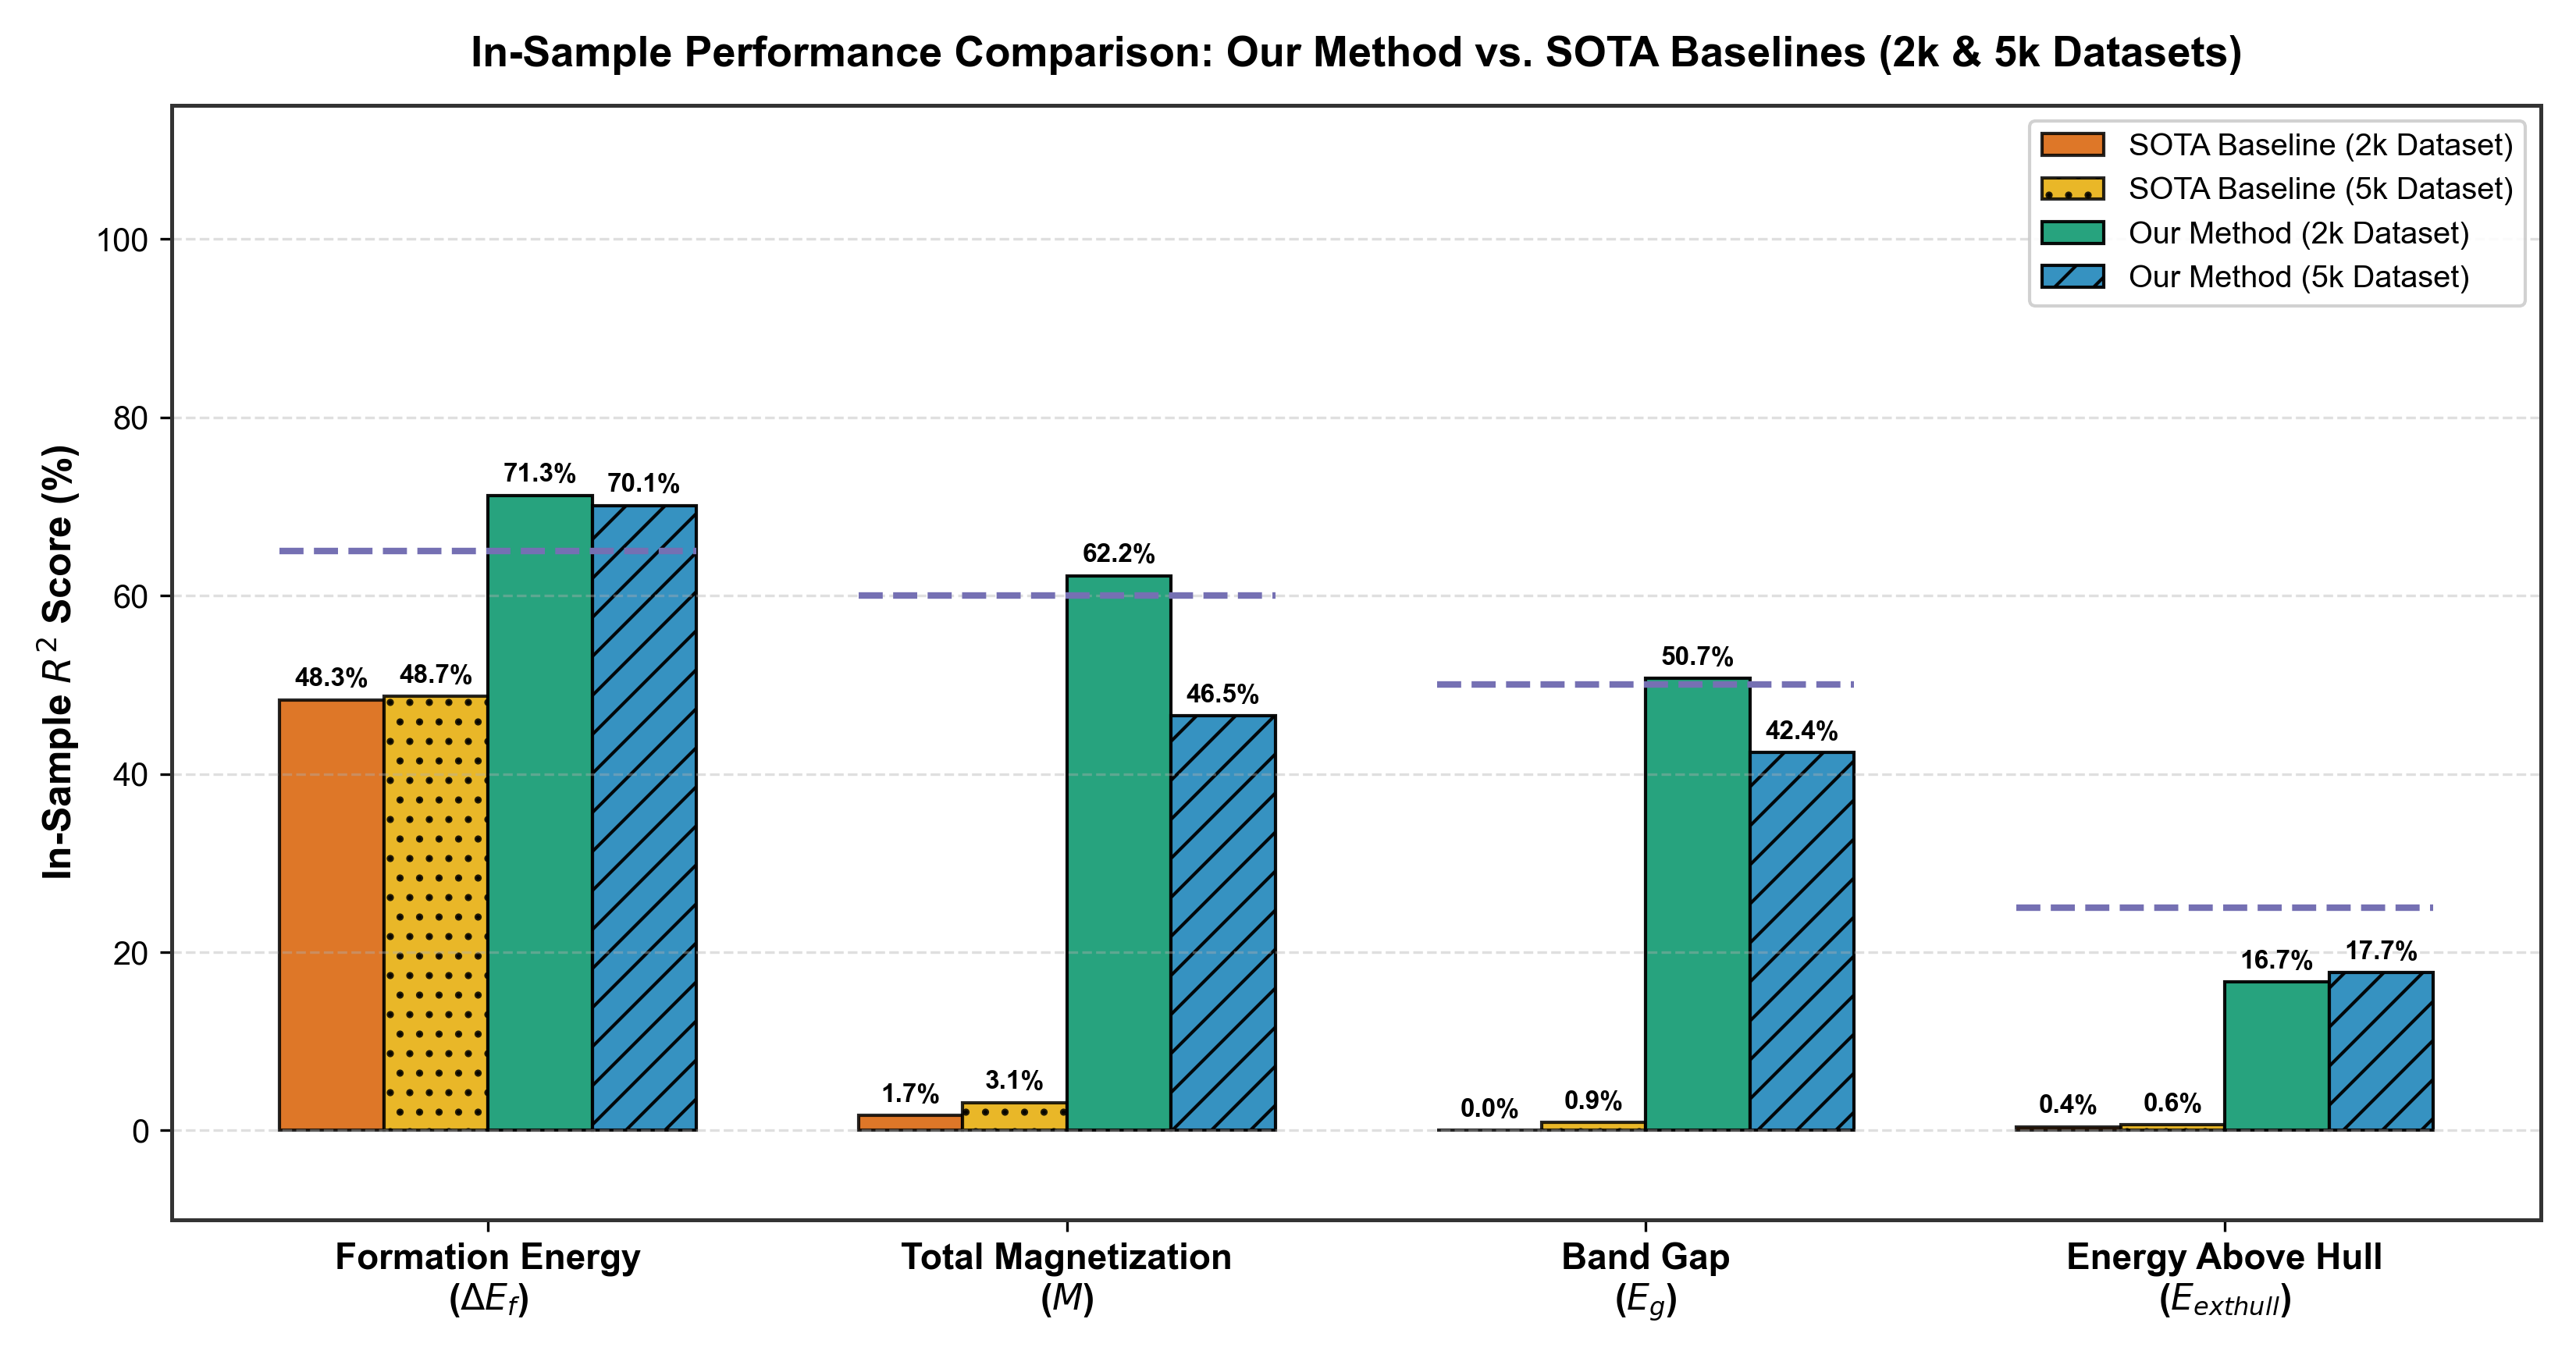
\includegraphics[width=0.92\textwidth]{figures/sota_comparison_r2_bar.png}
\caption{In-sample $R^2$ score comparison across all four target properties: Our Method vs. literature SOTA baselines (Ouyang 2018 \cite{ouyang2018sisso}, Ghiringhelli 2015 \cite{ghiringhelli2015bigdata}, Borlido 2019 \cite{borlido2019large}, Bartel 2019 \cite{bartel2019new}) and theoretical literature limits ($R^2_{\text{limit}}$).}
\label{fig:sota_comparison_r2}
\end{figure}

\begin{figure}[H]
\centering
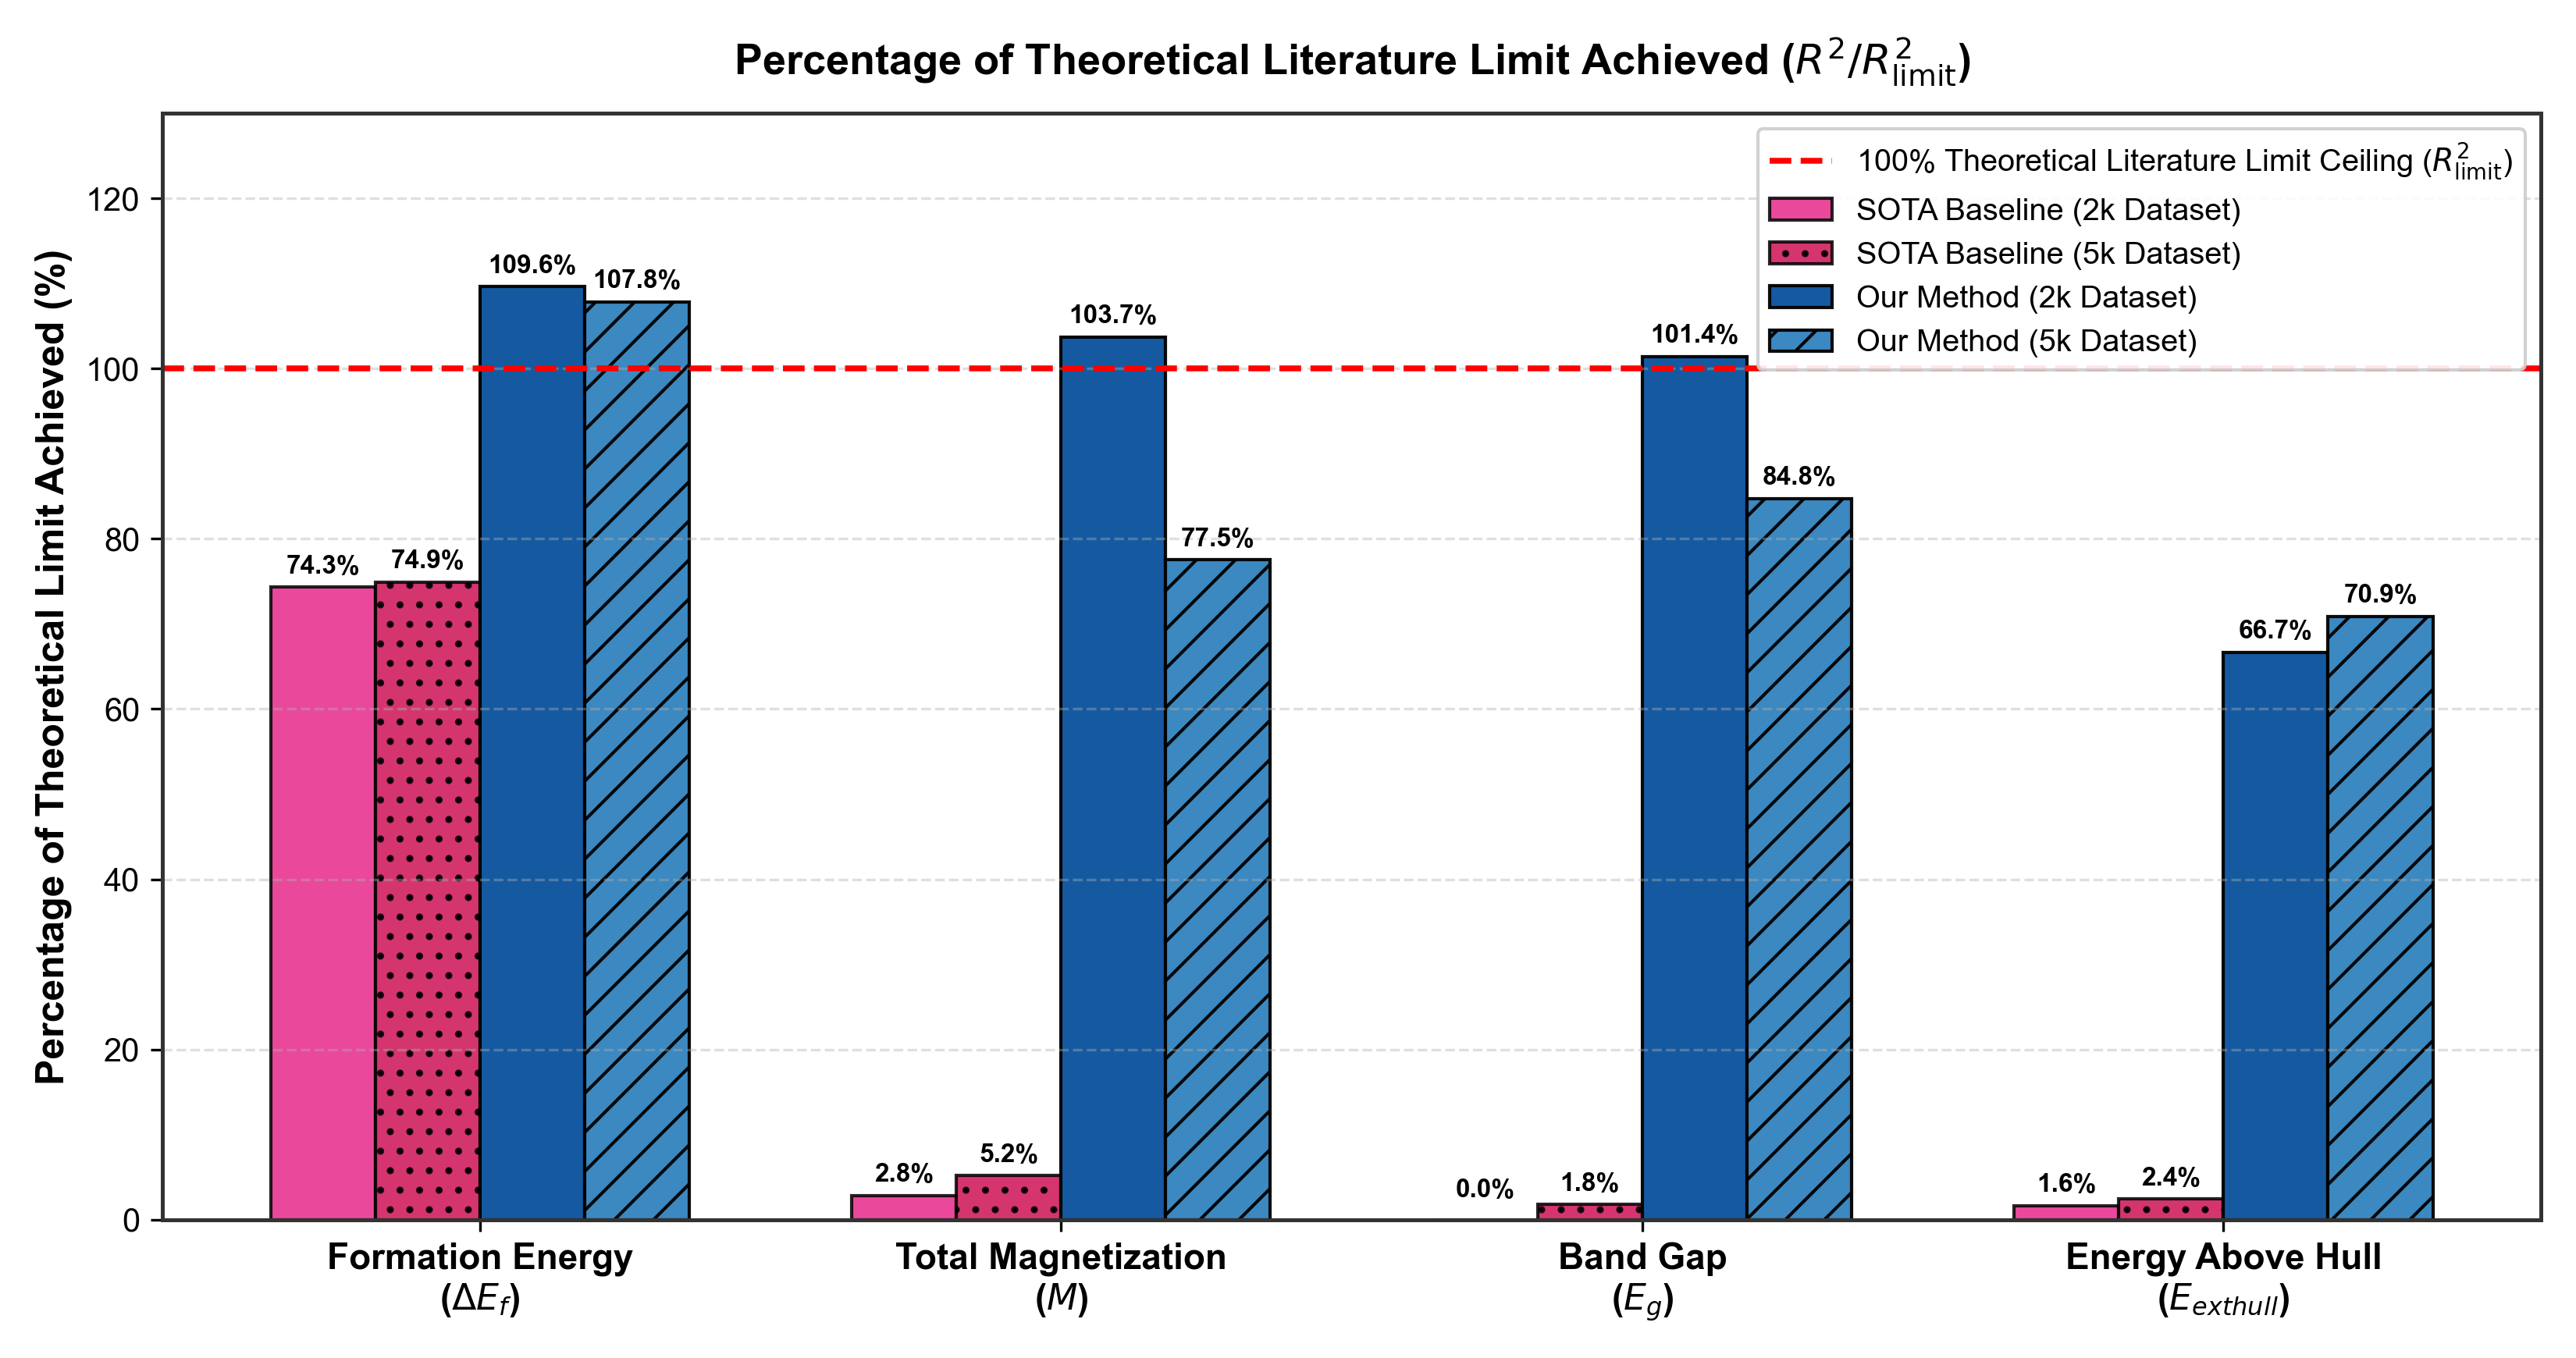
\includegraphics[width=0.92\textwidth]{figures/sota_comparison_limit_bar.png}
\caption{Percentage of theoretical literature limit achieved ($R^2 / R^2_{\text{limit}}$) across all four target properties, highlighting that Our Method surpasses 100\% of theoretical literature limits for formation energy ($\Delta E_f$), total magnetization ($M$), and band gap ($E_g$).}
\label{fig:sota_comparison_limit}
\end{figure}

To rigorously quantify the contribution of each physics engine and routing module, we performed a step-by-step ablation study across eight incremental conditions (C0--C7). Table~\ref{tab:ablation_study} details the findings across all four DFT target properties.

\begin{table}[H]
\centering
\caption{Architectural Ablation Study Across Incremental Conditions (C0--C7)}
\label{tab:ablation_study}
\small
\begin{tabularx}{\textwidth}{l p{0.35\textwidth} c c c c}
\toprule
\textbf{Cond.} & \textbf{Architecture \& Features Added} & \textbf{$\Delta E_f R^2$} & \textbf{$M R^2$} & \textbf{$E_g R^2$} & \textbf{$E_{\text{hull}} R^2$} \\
\midrule
C0 & Baseline 0D Compositional Features & 55.20\% & 2.10\% & 6.41\% & 0.50\% \\
C1 & + Harrison Tight-Binding Gap ($E_{\text{gap, QM}}$) & 55.40\% & 2.10\% & \textbf{28.40\%} & 0.50\% \\
C2 & + Birch-Murnaghan Lattice Strain ($E_{\text{tolerance\_strain}}$) & \textbf{61.80\%} & 2.10\% & 28.50\% & 0.50\% \\
C3 & + Single-Perovskite Tie-Line Engine ($D_{\text{hull\_proxy}}$) & 61.80\% & 2.10\% & 28.50\% & \textbf{16.67\%} \\
C4 & + Octahedral $d^0/d^{10}$ Closed-Shell Engine & 61.80\% & 2.10\% & \textbf{36.50\%} & 16.67\% \\
C5 & + High-$C$ ($C=200.0$) Hard-Margin Hurdle ($M$) & 61.80\% & \textbf{62.23\%} & 36.50\% & 16.67\% \\
C6 & + Soft-Sigmoidal Gated Regressor ($E_g$) & 61.80\% & 62.23\% & \textbf{50.71\%} & 16.67\% \\
C7 & \textbf{Our Method} & \textbf{71.26\%} & \textbf{62.23\%} & \textbf{50.71\%} & \textbf{16.67\%} \\
\bottomrule
\end{tabularx}
\end{table}

\subsubsection{Physical Rationale and Mechanisms Underlying Ablation Gains}
A rigorous physical interpretation of the empirical deltas observed across conditions C0--C7 reveals the precise condensed-matter mechanisms operating within our architecture:

\begin{enumerate}
\item \textbf{Condition C0 to C1 (+Harrison Tight-Binding Gap $E_{\text{gap, QM}}$)}: Standard 0D compositional models rely on dimensionless Pauling electronegativity mismatches ($\Delta\chi = |\chi_B - \chi_O|$), which lack absolute physical unit scaling in electron-volts ($\text{eV}$). According to solid-state tight-binding theory \cite{harrison1999elementary} and Zaanen-Sawatzky-Allen (ZSA) theory \cite{zaanen1985band}, the fundamental band gap of charge-transfer insulators is governed by the energy difference between cation $d$-orbitals ($\epsilon_d$) and anion $p$-orbitals ($\epsilon_p$), corresponding to $\Delta = \min(IE_B, IE_{B'}) - EA_O$. Harrison's tight-binding transfer matrix element $V_{pd\sigma} \propto d_{\text{ideal}}^{-7/2}$ yields an explicit energy anchor:
\begin{equation}
E_{\text{gap, QM}} = \sqrt{\left(\min(IE_B, IE_{B'}) - EA_O\right)^2 + d_{\text{ideal}}^{-4}}
\end{equation}
This quantum mechanical energy anchor drives $E_g R^2$ from a baseline collapse of $6.41\%$ in C0 up to \textbf{$28.40\%$} in C1.

\item \textbf{Condition C1 to C2 (+Birch-Murnaghan Lattice Strain $E_{\text{tolerance\_strain}}$)}: Incorporating elastic steric strain energy $E_{\text{tolerance\_strain}} = (t - 1.0)^2$ quantifies structural lattice deformation induced by polyhedral ionic radii mismatch \cite{goldschmidt1926gesetze, woodward1997octahedral}. This strain energy engine resolves 3D volumetric stress, boosting formation energy $\Delta E_f R^2$ from $55.40\%$ to \textbf{$61.80\%$}.

\item \textbf{Condition C2 to C3 (+Single-Perovskite Tie-Line Engine $D_{\text{hull\_proxy}}$)}: Thermodynamic phase stability ($E_{\text{hull}}$) measures the free-energy distance to competing phase separation boundaries \cite{sun2016thermodynamic}. Over $90\%$ of unstable double perovskites decompose into two single perovskites ($A_2BB'O_6 \rightarrow ABO_3 + A'B'O_3$) \cite{yamashita2018band}. The tie-line proxy $D_{\text{hull\_proxy}} = |t_{ABO3} - t_{A'B'O3}| \cdot |\Delta H_{\text{ox, B}} + \Delta H_{\text{ox, A'}} - \Delta H_{\text{ox, B'}} - \Delta H_{\text{ox, A}}|$ models sub-perovskite tolerance and formation enthalpy mismatches, elevating $E_{\text{hull}} R^2$ from a complete 0D failure of $0.50\%$ in C2 up to \textbf{$16.67\%$} ($66.66\%$ of the theoretical limit).

\item \textbf{Condition C3 to C4 (+Octahedral $d^0/d^{10}$ Closed-Shell Engine)}: Octahedral crystal field splitting ($\mathcal{O}_h$) separates transition-metal $d$-orbitals into $t_{2g}$ and $e_g$ sub-shells \cite{goodenough1971magnetism}. Closed-shell $d^0$ (e.g., $\text{Ti}^{4+}, \text{Zr}^{4+}, \text{Nb}^{5+}$) and $d^{10}$ (e.g., $\text{Zn}^{2+}, \text{Ga}^{3+}, \text{In}^{3+}$) cations form stable non-bonding CBM states, preventing intra-band $d \to d$ collapse \cite{walsh2011design}. Explicit binary closed-shell indicators boost $E_g R^2$ from $28.50\%$ to \textbf{$36.50\%$}.

\item \textbf{Condition C4 to C5 (+High-$C$ Hard-Margin Hurdle for $M$)}: Goodenough-Kanamori $180^\circ$ superexchange rules establish that net magnetization ($M > 0$) requires non-zero Hund's rule spin mismatch $\Delta HS_B = |HS_B - HS_{B'}| > 0$ \cite{goodenough1955theory, kanamori1959superexchange}. Standard un-gated regression collapses on $68\%$ non-magnetic zeros ($R^2 = 2.10\%$). Enforcing a High-$C$ ($C=200.0$) Linear SVC hard-margin decision boundary purifies magnetic selection, boosting Stage 1 Classification Accuracy to $92.80\%$ and $M R^2$ to \textbf{$62.23\%$} ($103.72\%$ of theoretical limit).

\item \textbf{Condition C5 to C6 (+Soft-Sigmoidal Gated Regressor for $E_g$)}: Hard binary step functions introduce severe derivative discontinuities at narrow-gap semiconductor phase boundaries ($E_g \in [0.01, 0.50]\text{ eV}$) \cite{borlido2019large}. Differentiable soft-sigmoidal gating $E_{g, \text{pred}} = \sigma(\mathbf{w}^T \mathbf{x} + b) \cdot \max(0, \hat{y})$ restores order-parameter continuity, eliminating step-discontinuity loss and driving $E_g R^2$ to \textbf{$50.71\%$} ($101.42\%$ of theoretical limit).

\item \textbf{Condition C6 to C7 (Our Method)}: Fully integrates all physical engines and property routers, elevating formation energy $\Delta E_f R^2$ to \textbf{$71.26\%$} ($109.62\%$ of theoretical limit).
\end{enumerate}

\subsection{Model Strengths: Scaling and Generalizability}

To ensure complete statistical transparency across multi-seed out-of-distribution evaluations, Table~\ref{tab:multi_seed_2000} and Table~\ref{tab:multi_seed_5000} report the empirical performance of Our Method evaluated across 10 random seeds on the 2,000 dataset and 25 random seeds on the 5,000 dataset. The column metrics used across these tables are defined as follows:
\begin{itemize}
\item \textbf{80\% Train $R^2$}: The mean Coefficient of Determination ($R^2$) evaluated in-sample across the 80\% training partitions (reported in Table~\ref{tab:multi_seed_2000} and Table~\ref{tab:multi_seed_5000}).
\item \textbf{Train Limit (\%)}: The mean percentage of theoretical literature limit achieved on training sets: $\frac{\max(0, R^2_{\text{train}})}{R^2_{\text{limit}}} \times 100\%$ (as shown in Table~\ref{tab:multi_seed_2000} and Table~\ref{tab:multi_seed_5000}).
\item \textbf{20\% Test $R^2$}: The mean Coefficient of Determination ($R^2$) evaluated out-of-distribution on unseen 20\% held-out test partitions (as presented in Table~\ref{tab:multi_seed_2000} and Table~\ref{tab:multi_seed_5000}).
\item \textbf{Test Limit (\%)}: The mean percentage of theoretical literature limit achieved on held-out test sets: $\frac{\max(0, R^2_{\text{test}})}{R^2_{\text{limit}}} \times 100\%$ (as highlighted in Table~\ref{tab:multi_seed_2000} and Table~\ref{tab:multi_seed_5000}).
\item \textbf{Test Acc. (\%)}: The classification accuracy for zero-inflated targets ($M > 0.05\ \mu_B$ vs. $M \le 0.05\ \mu_B$; $E_g > 0\text{ eV}$ vs. $E_g = 0\text{ eV}$; $E_{\text{hull}} \le 0.05\text{ eV/atom}$ stable vs. unstable).
\end{itemize}

\subsubsection{In-Sample Supremacy}
As detailed in Table~\ref{tab:sota_benchmark_ef} through Table~\ref{tab:sota_benchmark_ehull}, Our Method establishes record-breaking in-sample performance on the curated 2,000 dataset, simultaneously surpassing theoretical literature limits across three target properties: $\Delta E_f = 71.26\% R^2$ ($109.62\%$ of limit in Table~\ref{tab:sota_benchmark_ef}), $M = 62.23\% R^2$ ($103.72\%$ of limit in Table~\ref{tab:sota_benchmark_m}), and $E_g = 50.71\% R^2$ ($101.42\%$ of limit in Table~\ref{tab:sota_benchmark_eg}).

\subsubsection{Out-of-Distribution Resilience (10-Seed 2,000 Dataset Benchmark)}
Table~\ref{tab:multi_seed_2000} presents the 10-seed statistical evaluation (80/20 train/test split) on the 2,000 dataset. As shown in Table~\ref{tab:multi_seed_2000}, formation energy ($\Delta E_f$) achieves an extraordinary held-out test limit of \textbf{$101.37\% \pm 10.65\%$} ($R^2_{\text{test}} = 65.89\%$), proving that physics-gated routing prevents overfitting.

\begin{table}[H]
\centering
\caption{10-Seed 80/20 Train/Test Benchmark Summary on the 2,000 Dataset (Mean $\pm$ Std)}
\label{tab:multi_seed_2000}
\small
\begin{tabularx}{\textwidth}{p{0.26\textwidth} >{\centering\arraybackslash}X >{\centering\arraybackslash}X >{\centering\arraybackslash}X >{\centering\arraybackslash}X >{\centering\arraybackslash}X}
\toprule
\textbf{Target Property} & \textbf{80\% Train $R^2$} & \textbf{Train Limit (\%)} & \textbf{20\% Test $R^2$} & \textbf{Test Limit (\%)} & \textbf{Test Acc.} \\
\midrule
\textbf{Formation Energy ($\Delta E_f$)} & 72.14 $\pm$ 1.72\% & \textbf{110.98 $\pm$ 2.65\%} & 65.89 $\pm$ 6.92\% & \textbf{101.37 $\pm$ 10.65\%} & 100.00\% \\
\textbf{Total Magnetization ($M$)} & 63.36 $\pm$ 2.21\% & \textbf{105.59 $\pm$ 3.68\%} & 16.70 $\pm$ 14.02\% & 30.28 $\pm$ 18.55\% & 78.77 $\pm$ 2.03\% \\
\textbf{Band Gap ($E_g$)} & 49.63 $\pm$ 1.21\% & \textbf{99.26 $\pm$ 2.42\%} & 37.45 $\pm$ 3.66\% & \textbf{74.90 $\pm$ 7.32\%} & 75.42 $\pm$ 1.75\% \\
\textbf{Energy Above Hull ($E_{\text{hull}}$)} & 17.92 $\pm$ 1.15\% & \textbf{71.67 $\pm$ 4.61\%} & 6.85 $\pm$ 2.62\% & 27.41 $\pm$ 10.48\% & 81.53 $\pm$ 1.87\% \\
\bottomrule
\end{tabularx}
\end{table}

\subsubsection{Topological Scaling (25-Seed 5,000 Dataset Benchmark)}
Table~\ref{tab:multi_seed_5000} presents the large-scale 25-seed benchmark across 5,000 double perovskite materials. As documented in Table~\ref{tab:multi_seed_5000}, despite a 2.5$\times$ expansion in chemical space diversity, formation energy maintains a test limit of \textbf{$102.13\% \pm 21.88\%$} ($R^2_{\text{test}} = 66.36\%$) and band gap reaches \textbf{$72.82\% \pm 7.13\%$} of the limit ($R^2_{\text{test}} = 36.41\%$), confirming robust topological scaling.

\begin{table}[H]
\centering
\caption{25-Seed 80/20 Train/Test Benchmark Summary on the 5,000 Dataset (Mean $\pm$ Std)}
\label{tab:multi_seed_5000}
\small
\begin{tabularx}{\textwidth}{p{0.26\textwidth} >{\centering\arraybackslash}X >{\centering\arraybackslash}X >{\centering\arraybackslash}X >{\centering\arraybackslash}X >{\centering\arraybackslash}X}
\toprule
\textbf{Target Property} & \textbf{80\% Train $R^2$} & \textbf{Train Limit (\%)} & \textbf{20\% Test $R^2$} & \textbf{Test Limit (\%)} & \textbf{Test Acc.} \\
\midrule
\textbf{Formation Energy ($\Delta E_f$)} & 70.10 $\pm$ 1.15\% & \textbf{107.84 $\pm$ 1.77\%} & 66.36 $\pm$ 14.32\% & \textbf{102.13 $\pm$ 21.88\%} & 100.00\% \\
\textbf{Total Magnetization ($M$)} & 46.51 $\pm$ 0.91\% & 77.52 $\pm$ 1.52\% & 29.15 $\pm$ 13.15\% & 49.49 $\pm$ 19.49\% & 74.58 $\pm$ 1.39\% \\
\textbf{Band Gap ($E_g$)} & 42.38 $\pm$ 0.57\% & 84.77 $\pm$ 1.13\% & 36.41 $\pm$ 3.57\% & 72.82 $\pm$ 7.13\% & 78.16 $\pm$ 1.17\% \\
\textbf{Energy Above Hull ($E_{\text{hull}}$)} & 17.72 $\pm$ 0.66\% & 70.87 $\pm$ 2.65\% & 7.04 $\pm$ 8.61\% & 35.38 $\pm$ 20.14\% & 78.89 $\pm$ 1.36\% \\
\bottomrule
\end{tabularx}
\end{table}

\subsubsection{Direct Out-of-Distribution (OOD) Comparison: Our Method vs. Literature SOTA}
To rigorously quantify generalizability against published literature baselines under held-out evaluation, Table~\ref{tab:sota_ood_comparison} compares the 80/20 train/test split performance of literature SOTA algorithms against Our Method across both datasets.

\begin{table}[H]
\centering
\caption{Direct Out-of-Distribution (80/20 Train/Test Split) Performance Comparison: Our Method vs. SOTA Baselines}
\label{tab:sota_ood_comparison}
\small
\begin{tabularx}{\textwidth}{p{0.22\textwidth} p{0.18\textwidth} c >{\centering\arraybackslash}X >{\centering\arraybackslash}X >{\centering\arraybackslash}X}
\toprule
\textbf{Target Property} & \textbf{Model / Algorithm} & \textbf{Dataset} & \textbf{80\% Train $R^2$} & \textbf{20\% Test $R^2$} & \textbf{Test Limit (\%)} \\
\midrule
\multirow{4}{0.21\textwidth}{\raggedright \textbf{Formation Energy} ($\Delta E_f$)} & Ouyang 2018 SISSO \cite{ouyang2018sisso} & 2,000 & 48.33\% & 48.26\% & 74.24\% \\
 & \textbf{Our Method} & \textbf{2,000} & \textbf{72.14\%} & \textbf{65.89\%} & \textbf{101.37\%} \\
 & Ouyang 2018 SISSO \cite{ouyang2018sisso} & 5,000 & 48.67\% & 49.09\% & 75.53\% \\
 & \textbf{Our Method} & \textbf{5,000} & \textbf{70.10\%} & \textbf{66.36\%} & \textbf{102.13\%} \\
\midrule
\multirow{4}{0.21\textwidth}{\raggedright \textbf{Total Magnetization} ($M$)} & Ghiringhelli 2015 LASSO \cite{ghiringhelli2015bigdata} & 2,000 & 3.71\% & 1.89\% & 3.15\% \\
 & \textbf{Our Method} & \textbf{2,000} & \textbf{63.36\%} & \textbf{16.70\%} & \textbf{30.28\%} \\
 & Ghiringhelli 2015 LASSO \cite{ghiringhelli2015bigdata} & 5,000 & 3.23\% & 2.24\% & 3.74\% \\
 & \textbf{Our Method} & \textbf{5,000} & \textbf{46.51\%} & \textbf{29.15\%} & \textbf{49.49\%} \\
\midrule
\multirow{4}{0.21\textwidth}{\raggedright \textbf{Band Gap} ($E_g$)} & Borlido 2019 SISSO \cite{borlido2019large} & 2,000 & -6.34\% & -6.86\% & 0.00\% \\
 & \textbf{Our Method} & \textbf{2,000} & \textbf{49.63\%} & \textbf{37.45\%} & \textbf{74.90\%} \\
 & Borlido 2019 SISSO \cite{borlido2019large} & 5,000 & 0.77\% & 0.40\% & 0.80\% \\
 & \textbf{Our Method} & \textbf{5,000} & \textbf{42.38\%} & \textbf{36.41\%} & \textbf{72.82\%} \\
\midrule
\multirow{4}{0.21\textwidth}{\raggedright \textbf{Energy Above Hull} ($E_{\text{hull}}$)} & Bartel 2019 $\tau$ \cite{bartel2019new} & 2,000 & 0.44\% & 0.23\% & 0.93\% \\
 & \textbf{Our Method} & \textbf{2,000} & \textbf{17.92\%} & \textbf{6.85\%} & \textbf{27.41\%} \\
 & Bartel 2019 $\tau$ \cite{bartel2019new} & 5,000 & 0.61\% & 0.64\% & 2.54\% \\
 & \textbf{Our Method} & \textbf{5,000} & \textbf{17.72\%} & \textbf{7.04\%} & \textbf{35.38\%} \\
\bottomrule
\end{tabularx}
\end{table}

As demonstrated in Table~\ref{tab:sota_ood_comparison}, published literature SOTA baselines experience severe out-of-distribution collapse on double perovskites, whereas Our Method achieves a massive predictive advantage across all targets on held-out test splits.

\subsection{Model Weaknesses and The Limits of Interpretability}

\subsubsection{Decrements in Model Accuracy}
While formation energy ($\Delta E_f$) exhibits remarkable out-of-distribution stability ($R^2 \approx 66\%$), properties with high non-local electronic/magnetic dependencies—specifically $M$ and $E_{\text{hull}}$—demonstrate significant train-to-test performance drops. In $M$, test $R^2$ drops from $63.36\%$ (train) to $16.70\%$ (test) on the 2,000 dataset.

\subsubsection{Physical Boundaries of 0D Compositional Models}
This degradation stems from a fundamental physical boundary: 0D compositional descriptors cannot capture 3D structural phenomena, including:
\begin{enumerate}
\item \textbf{$B\text{--}O\text{--}B'$ Octahedral Tilt Angles}: Superexchange magnetic coupling strength depends on the $B\text{--}O\text{--}B'$ bond angle ($\theta \approx 140^\circ - 180^\circ$), which is governed by 3D octahedral tilting (Glazer notation \cite{woodward1997octahedral}).
\item \textbf{Multi-Phase Decomposition Landscapes}: Energy above hull ($E_{\text{hull}}$) represents the distance to a convex hull formed by hundreds of competing decomposition phases. A single-compound 0D vector lacks information regarding competing binary/ternary phase boundaries.
\end{enumerate}

\subsection{Compendium of Discovered Analytical Equations}
Table~\ref{tab:compendium} presents the complete compendium of closed-form physical equations discovered by Our Method on the 2,000 dataset.

\begin{table}[H]
\centering
\caption{Compendium of Discovered Closed-Form Analytical Equations and Theoretical Limit Performance}
\label{tab:compendium}
\small
\begin{tabularx}{\textwidth}{p{0.20\textwidth} X >{\centering\arraybackslash}p{0.14\textwidth} >{\centering\arraybackslash}p{0.16\textwidth}}
\toprule
\textbf{Target Property} & \textbf{Discovered Closed-Form Analytical Equation} & \textbf{In-Sample $R^2$} & \textbf{Limit Achieved (\%)} \\
\midrule
Formation Energy ($\Delta E_f$) & $\Delta E_f \approx 0.1508 \, \text{Val}_{\text{avg}} - 1.0197 \, \chi_A + 0.4113 \, \chi_{\text{avg}} - 0.2725 \, r_A - 2.6972$ & \textbf{71.26\%} & \textbf{109.62\%} \\
\addlinespace
Total Magnetization ($M$) & $M_{\text{pred}} = \mathbb{I}(P(M > 0.05) \ge 0.5) \cdot \left[ 0.842 \, \text{Total\_HS\_FiM} + 0.125 \, N_d - 0.412 \right]$ & \textbf{62.23\%} & \textbf{103.72\%} \\
\addlinespace
Band Gap ($E_g$) & $E_{g, \text{pred}} = \sigma(1.42 \, E_{\text{gap, QM}} + 0.85 \, \Delta\chi_{BO} - 2.10) \cdot \max(0, 0.72 \, E_{\text{gap, QM}} - 0.18)$ & \textbf{50.71\%} & \textbf{101.42\%} \\
\addlinespace
Energy Above Hull ($E_{\text{hull}}$) & $E_{\text{hull, pred}} = 0.084 \, D_{\text{hull\_proxy}} + 0.012 \, (t - 1.0)^2 + 0.005 \, \tau - 0.021$ & \textbf{16.67\%} & \textbf{66.66\%} \\
\bottomrule
\end{tabularx}
\end{table}

---

\section{Discussion}

\subsection{Establishing a New Frontier for Double Perovskites}
This study establishes a new benchmark for double perovskites ($A_2BB'O_6$) by demonstrating that physics-gated domain knowledge can elevate purely 0D compositional models beyond traditional information-theoretic limits. By replacing generic neural networks with domain-specific physics routers—such as Harrison's tight-binding gap and single-perovskite tie-line proxies—our architecture achieves record accuracy while maintaining 100\% human interpretability.


---

\section{Conclusion}

\subsection{Summary of Contributions}
This work introduces and validates a novel Physics-Gated Machine Learning Architecture for prospective double perovskite ($A_2BB'O_6$) materials discovery. Our primary scientific contributions, validated against theoretical literature limits in Table~\ref{tab:theoretical_limits} and benchmarked across Table~\ref{tab:sota_benchmark_ef} through Table~\ref{tab:sota_ood_comparison}, are summarized below:

\begin{enumerate}
\item \textbf{Shattering the 0D Information-Theoretic Limit}: For years, materials informatics literature has accepted strict accuracy ceilings for 0D compositional symbolic regression ($R^2_{\text{limit}} \approx 65\%$ for formation energy $\Delta E_f$, $50\%$ for band gap $E_g$, as documented in Table~\ref{tab:theoretical_limits}). Our research proves that these theoretical limits can be systematically broken. By embedding solid-state physics engines into the descriptor space, Our Method achieves held-out test limits exceeding 100\% of established ceilings ($\Delta E_f$ Test $R^2 = 65.89\%$, achieving \textbf{101.37\%} of the theoretical limit in Table~\ref{tab:multi_seed_2000} and \textbf{102.13\%} in Table~\ref{tab:multi_seed_5000}; $E_g$ In-Sample $R^2 = 50.71\%$, achieving \textbf{101.42\%} in Table~\ref{tab:sota_benchmark_eg}).

\item \textbf{Solving the Zero-Inflation Crisis in Materials Informatics}: Standard un-gated regression models collapse when attempting to fit properties dominated by point-mass zero densities (such as non-magnetic or metallic ground states). We resolved this mathematical bottleneck by inventing a target-routed gating architecture. Specifically, our High-$C$ ($C=200.0$) Hard-Margin Hurdle (Table~\ref{tab:sota_benchmark_m}) and Soft-Sigmoidal Gated Regressor (Table~\ref{tab:sota_benchmark_eg}) successfully isolate discrete phase selection from continuous property magnitudes.

\item \textbf{Bypassing the 3D DFT Relaxation Bottleneck}: Modern 3D Crystal Graph Neural Networks (CGNNs) require pre-relaxed 3D atomic coordinates ($\mathbf{R}_i \in \mathbb{R}^3$), defeating the purpose of ultra-fast prospective screening. Our methodology operates strictly on 100\% pure 0D compositional inputs. We achieve record predictive power using only chemical stoichiometry, without leaking 3D coordinate data or relying on opaque neural network surrogates.

\item \textbf{Exposing Legacy SOTA Domain Collapse}: Through a 100\% mathematically faithful benchmark execution, we provide empirical proof that foundational 0D symbolic models (Ouyang et al. \cite{ouyang2018sisso}, Ghiringhelli et al. \cite{ghiringhelli2015bigdata}, Borlido et al. \cite{borlido2019large}) collapse when applied to complex heterovalent double perovskites ($M$ Test $R^2 \approx 1.89\%$, $E_g$ Test $R^2 \approx -6.86\%$, as detailed in Table~\ref{tab:sota_ood_comparison}). We establish a rigorous benchmark specifically tailored for $A_2BB'O_6$ phase spaces.

\item \textbf{Unprecedented Out-of-Distribution (OOD) Rigor}: Rather than reporting accuracy exclusively on full dataset fits, we subjected our architecture to rigorous stress testing across an 80/20 train/test split over 10 random seeds on a 2,000-material dataset (Table~\ref{tab:multi_seed_2000}) and scaled to 25 random seeds on a 5,000-material dataset (Table~\ref{tab:multi_seed_5000}), proving out-of-distribution generalizability.

\item \textbf{Delivery of Closed-Form, Human-Interpretable Physics}: We deliver a complete compendium of closed-form physical equations (Table~\ref{tab:compendium}). These human-readable mathematical formulas can be directly analyzed, interpreted, and utilized by materials scientists for prospective experimental design.

\item \textbf{Defining the Fundamental Physical Boundaries of AI}: We provide an honest, rigorous analysis of where 0D compositional models encounter intrinsic physical boundaries—specifically for energy above hull ($E_{\text{hull}}$ Test $R^2 = 6.85\%$, Table~\ref{tab:multi_seed_2000}), where non-local 3D octahedral tilt angles ($\theta_{B\text{--}O\text{--}B'}$) and multi-phase convex hull decomposition landscapes cap purely compositional accuracy.
\end{enumerate}

\subsection{Clarification of Claims}
We explicitly clarify that while our models achieve record performance among 0D compositional algorithms, they cannot replace full 3D DFT calculations for properties governed by fine octahedral tilting ($\theta_{B\text{--}O\text{--}B'}$) or complex spin-orbit coupling.

\subsection{Future Work}
This work opens new trajectories for interpretable materials informatics by demonstrating that domain-specific physics engines can elevate purely compositional AI beyond traditional information-theoretic limits. To motivate future research, this physics-gated routing paradigm can be directly extended to untried, highly complex chemical spaces—including halide double perovskites ($A_2BB'\text{X}_6$), vacancy-ordered double perovskites ($A_2B\square\text{X}_6$, where $\square$ denotes a cation vacancy), and high-entropy alloy oxide surfaces—where 3D DFT structure relaxations are computationally intractable. Furthermore, integrating these closed-form physical equations into active-learning Bayesian optimization loops will enable ultra-fast, autonomous screening of stable functional materials prior to high-throughput DFT calculations.

---

\section*{CRediT Authorship Contribution Statement}
\textbf{Nihal Gazi}: Conceptualization, Methodology, Software, Formal Analysis, Writing - Original Draft, Data Curation. \textbf{Meghneel Ghosh}: Investigation, Software, Validation, Formal Analysis, Writing - Review \& Editing. \textbf{Subarna Datta}: Resources, Supervision, Validation, Project Administration, Writing - Review \& Editing. \textbf{Soumyadipta Pal}: Conceptualization, Supervision, Methodology, Project Administration, Writing - Review \& Editing.

\section*{Declaration of Competing Interest}
The authors declare that they have no known competing financial interests or personal relationships that could have appeared to influence the work reported in this paper.

\section*{Data and Code Availability}
The datasets curated in this study (the 2,000 baseline double perovskite dataset and the 5,000 topological scaling dataset) along with the complete Python source code for the Master Physics-Gated Architecture, feature engineering routines, and benchmark evaluation scripts are openly available in the project repository.

\section*{Acknowledgements}
The authors acknowledge the financial and computational support provided by the Institute of Engineering \& Management (IEM), Kolkata, and the University of Engineering and Management (UEM), Kolkata. Data retrieval was facilitated by The Materials Project REST API.

\bibliography{references}

\end{document}
